\section{Chang\'E-4 and Lunar Lander Neutron and Dosimetry Experiment}
\label{sec:change_4_LND}

\subsection{Overview and current status (2019 - 2022)}

\begin{figure}
    \centering
    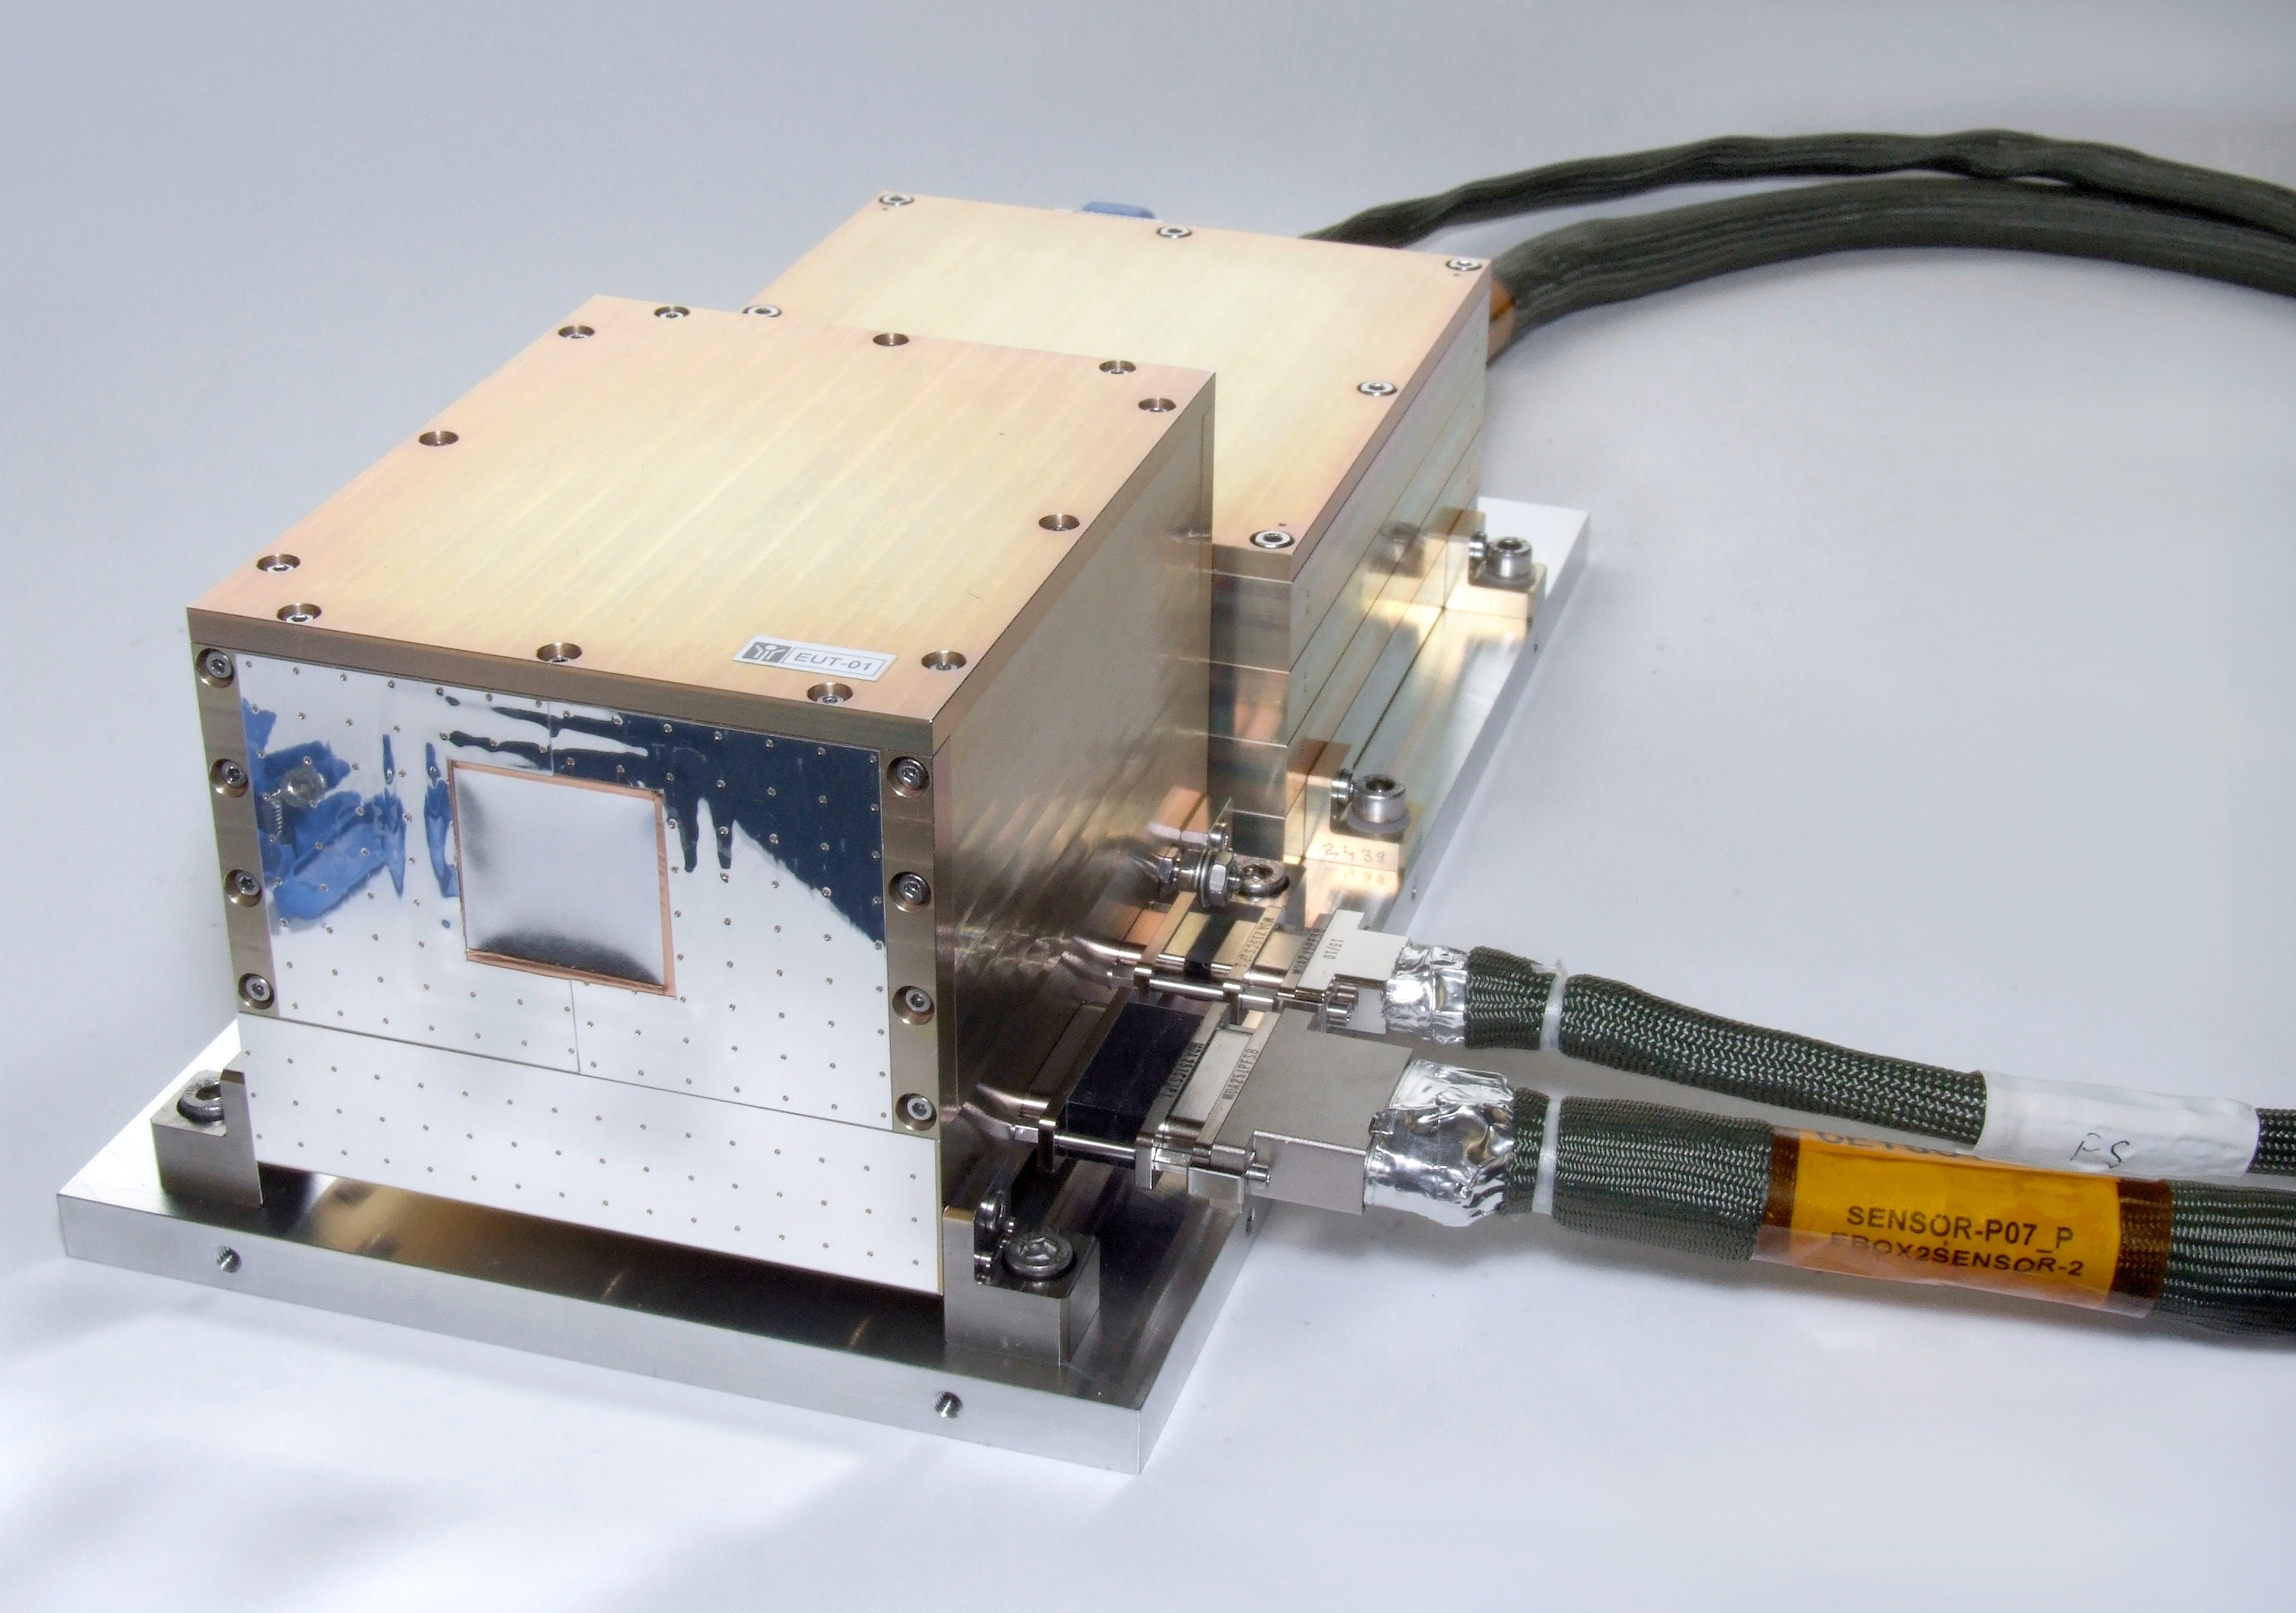
\includegraphics[width = 0.4\textwidth]{images/LND_2018-11-13.JPG}
    \caption{The photographs of LND instrument, including the sensor head (SH, front), and electronics box (EB, rear), and 1-meters data and powver harness that connects the SH and EB. The figure was from \cite{Wimmer-2020-LND} which is actually the flight spare model of LND and wass token on 2018-11-23 for the instrument paper}
    \label{Fig:LND_instrument}
\end{figure}

\begin{figure}
    \centering
    \includegraphics[width = 0.4\textwidth]{images/change4_lnd-c9_trigger-cones-colored.pdf}
    \caption{The skeptical view of the inner structure of the sensor head. Ten 500 $\mu$m silicon \acs{SSD} are assembly in order from A to J. The figure was from \cite{Wimmer-2020-LND}. More detailes could be found in the instrument paper.}
\end{figure}
Chang'E-4 is a chinese lunar exploration mission to the lunar far-side surface, which is also the first human mission sofely landed on the lunar far-side surface. The whole mission consists of a lander, a rover (Yutu-2, citaion) and a relay sattellite (Queqiao, citaion) which is working in the lunar orbit and responsible for the communication between the lunar far-side surface and the ground. The mission was launched on December 7, 2018 and successfully landed on January 3, 2019 in the Von K\`arm\`an crater near the south pole of Moon. 

There four 
including 4 international     al payloads and 4 domestic payloads.
Environment, 
Up to now.

As one of the four internation payload, LND is designed by  Kiel University
Which is a  instrument 
Aim at 
The main scientific objects of LND, as indicated in the instrument paper, are the following:
\begin{itemize}
    \item Dosimetry for human exploration of the Moon
    \item Contribution to the heliospheric science
\end{itemize}
And LND also has two technological demonstration objects which are \textit{Determine the subsurface water content in the South-Pole Aitken Basin} and \textit{Determine the FeO content in the South-Pole Aitken Basin} 
To achieve the above scientific objects, LND measure and provide the data products including up to 1-minute charged and neutral particle dose rate measured in Si, up to 1 minute cadence LET spectra, 1 minute neutral particle deposition energy spectra, 10 minute count rates of thermal neutrons and high time resolution (1-min, 10-min) flux and high energy resolution charged particle spectra including the electron and ions from proton to iron.


LND only working on the local day time of lunar farside. One of major challenge of LND on the lunar far-side surface is the 
The easiest way to check whether LND is working or not is looking up during night, if you see a ? moon, which indicates that moon is moving our of the earth's shawdown and the farside is facing the sun. Once the light is arriving at the lander, the system will be waken up and start to work. So is LND and other instruments.

Up to May 2023, LND has been working on the lunar far-side surface for more than 4 years (more then 50 Lunar days), already exceeding its designed life time. 

LND was switch off or switch on for a short period on the 6th, 44th, 45th lunar days, due to the special operations of lander and the extre movement from the ground. Up to May 2023, when the thesis finished, we have received the 46 lunar day data from January 2019 to the end of November 2022. The more data is coming. 
The data is officially publishing in the Lunar and Planetary Data release system \url{moon.bao.ac.cn}. An alternative way to download the data is from the PDS \url{https://pds.nasa.gov/}. The data is also available in the \ac{PSA} \url{https://psa.esac.esa.int/psa/}.

After LND delivered and launched, we implement several configuration changes and upload together 14 extra commands to fix the issues including the design issue and the malfunction issue. The design issue is due to the bugs in the processing software causing the wrong usage of the channels. The affection on the data products is minor. However, the major change of the data products are caused by the sky rocket of the noise level in certain channels. The reason for the noise issue is due to the unproper operation in the ground. On the 3rd and 4th lunar day, LND was switched off but kept the LND lid open until LND was switch shortly after. The immediately consequence of such operation is the dramastically drop of the temperature on the detector. Such a change is unrecoveryable, even if the temperature is back to normal.

To mitigating the impact of the noise issue and its influence on the data products, we implement several changes including raise the threshold of the noise detector, disable A2 channels which larger affect the LET spectra and hardly fixed by raising the threshold. No doubt, the consequence of such changes is obviouse. For instance, we lose the measurement of minimum ioninzing particle after the increment of the threshold of I detector, and the geometry factor of LET spectra and penetrating particle are dramatically reduced since we disable A outer channels. 

The details of the configuration changes and affections are given in the Appendix of chapter \ref{} and the corresponding change of the original code in the LND data processing software is given in the appendix ( if you have time to do it)

As we listed before, a major 


During the first half year of Chang'e-4 mission, the sun had a extremely quite phase and the solar activities reached the minimum level as indicated by the monthly averaged sunspot number which is nearly zero according to the observation from *****. Furthmmore, almost no SEP events happened during this period. 

On the other side, the crucial environment on the lunar far-side surface is a big challenge for the LND to work properly. The
The LND is designed to work in the temperature range of -40 to 60 degree, but the temperature on the lunar surface could be as low as -180 degree during the night.
In order to protect the detectors from the frozen temperature, the LND is only allowed to work during the day time after the lander is raised by the light of the sun.
During night, the RTG and RHU heater will keep the Lander and other scientific payload warm. 
Since LND only work 1\/3 of the time, the chance that LND encounter a SEP event during the solar minimum is even lower.

However, the LND is still lucky enough detecting several SEP events during the first half of 2019. 
On May 2019, two SEP events arrived on the lunar surface and 

\subsection{Charged particle telescope of LND}

The typical paragraph of the charged particle design and the measurement principle.



\subsection{dosimeter and neutron particle measurement}
Simple explain the desgin and the measurement principle.
And explain first result paper, background paper to determined the radiaion background



\subsection{Possible opportunity of the LND data}





\section{Solar orbiter and High energy telescope}

Launched on Feb 10, 2020, \acl{SolO}\acused{SolO} missions [citation] is an international mission cooperated between \ac{ESA} and \ac{NASA}. The aim of this mission is to understand the sun and how it control the so-called helisphere. As indicated in solo mission paper, the following scientifice questions will be answered and further studies:
\begin{itemize}
	\item 1
	\item 2
	\item 3
\end{itemize}
After finishing the cuise phase which started at June 14, 2020, currently, \ac{SolO} is operating as planned in the nominla mission phase since Nov 26, 2021.
The \ac{SolO} has a special designed elliptic helioscentric orbit with the closest perihelion of 0.29 AU (about 42$\times10^6$ km) in the whole mission. Using several gravity assistance during the venus flyby and earth flyby, the orbit of SolO will gradually tilt away from the ecliptic plane, in the end is 24 degrees above the Sun's equator.

Up to May 2023, when this thesis is drafted, \ac{SolO} is still following an elliptical orbit around the sun, with a maximum solar latitude of 8.66 degrees. \ac{SolO} has finished 5 perihelions with closest distance of 0.292 AU on Sep 3, 2022, and is starting its 6th orbit, moving on the way away the Sun. Three time Venus flyby happened on Dec 27, 2020,  Aug 9, 2021 and Sep 4, 2022. The Earth GAM happend on Now 27, 2021.

The above mentioned solo tragjectory information is taken from the \hyperlink{https://issues.cosmos.esa.int/solarorbiterwiki/display/SOSP/Trajectory+Overview+-+10+February+2020+Launch}{Solar orbiter Consolidated Report on Mission analysis}

Benefit from the special position of \ac{SolO} during this trip, the multiple scientific instrument onboard the \ac{SolO} coudl furtherly advanced the studies  in relative field and certain topic, for instance, remote- sensing [?], solar wind [?], SEP [?], GCR [?].

EPD [citation here]is one of such scientific payload suite onboard solo, aiming at the charge particles with energy spans over a large scale from few kev to few GeV,In this larger energy range, all the plasma population including lower energy solar wind,  $\sim$ kev suprathermal particle, high energy SEP, ACR and GCR are measured and studies.
EPD consists of four instruments, \ac{SIS}, is a time-of-flight mass spectrometer that measures ion composition from  $\sim$ 0.1 - few MeV
10 MeV nucleon$^{-1}$ designed by JPL; \ac{STEP}, is ? that measures what?;  \ac{EPT} is ? and measure ? and \ac{HET}, is what and measure what
Apart from SIS, all other instrument are design by Kiel group.
Those four instruments are assembly on the SolO as the Fig.{}explain the instrument together image. The energy coverage of those four instruments are shown in Fig.{EPD energy range}.

In the following section, we briefly introduce some details of the \ac{HET}, which is the mainly used in our study.

Overview
\subsection{High energy telescope}

The high energy telescopes (HET), as one of the scientific payload of The Energetic Particle Detector (EPD) \cite{EPD_instrument} on the Solar Orbiter, are designed to measure the high energetic particles and cover the higher end of the EPD energy range. The typical particles that HET measures include $\sim$ MeV electrons [citaion] and tens of MeV to few GeV positively charged particles like, protons, helium-4 and its isotope Helium-3, carbon, oxygen, nitrogen, and even heavy elements iron. 

Two HET units, HET1 and HET2, are equiped on the \ac{SolO}. They are specially mounted on two perpendicular direcitons, sun-asun (ecliptic) and south-north (polar), providing the angle information of particles in the interplanetary space[citatoin]. Such measurements are especially useful during the SEP event because the pitch angle  distribution of energetic paricle in the magnetic field is an important paramter to understand the transportation of particle [citaion, find precious words]. 

Each HET is a double-ended telescope which consists of four 300 $\mu$m silicon solid-state (SSD) detectors stacks, with two in each side (A1, B1 in the front side and A2, B2 in the back side), and a 2 cm thick $Bi_{4}Ge_{3}O_{12}$ (BGO) scintillator, in the center. The inner structure of the HET sensor head is given in Fig.\ref{fig:HET-sensor-head}. HET use the dE/dX - E technique to discriminates different particle species of different energy, including electron, proton, helium-4, and heavy ions like carbon, nitrogen, oxygen, and iron.  ( to expand and more details)



\begin{figure}
    \centering
    \includegraphics[width = 0.6\textwidth]{images/het.png}
    \caption{The sensor head o}
    \label{fig:HET-sensor-head}
\end{figure}



As given in Table 22 of \cite{EPD instruemnt},the nominal data products of HET include ABnC (6.5 - 9.5 Me\/nuc), ABC ($\sim$10 - $\sim$ 100 MeV/nuc) and penetrating (above 100 MeV/nuc). The energy range in the bracket are the designed energy range of helium-4 measurement by HET. In this study, we use the data products that measure helium stopping in inner C detector i.e. the ABC coincidence and we specially use the energy between 10 - 50 MeV\/nuc, because this is exactly the energy region where ACR helium dominate and the data product of SOHO\/EPHIN exaclty cover this energy region which we introduce in the following section. We will calculate the ratio of flux between HET and EPHIN. 
Besides, the lowest energy channels of ABnC coincidence have unsolved calibration issue and the measurement of remain channels are constrained by their counting statistics which result in a relatively larger uncertainties.



The nominal scientific data products of HET are designed to study SEP events of higher intensity by limiting the FOV and using coincidence measurements to discriminate species and achieve better energy resolution. However such data products are not optimal for the analysis that requires both time resolution and larger counting statistc, for instance to determine the SEP events period.    Alternatively, single detector count rates without any coincidence conditions which is one kind of housekeeping data, could provide the possibility to achieve better counting statistic. Von forstner et al 2021 use the single C counter to study the temporal varitation of the forbush decrease and Allen et al 2021 confirmed the drop out of C counter rate during the first venus flyby is due to the VENUS blockage on the HET FOV.

Similar with the single detector count rate, in the study, we introduce \textit{any(a1, b1)} which is a level-2 trigger of HET to determine the SEP period. \textit{a1} and \textit{b1} represent the front two SSDs of HET sensor head. This level-2 trigger counts all the particles that have energy above the threshold of detector A or detector B, which is 50 keV in the nominal mode [citaion effman thesis]. Since no obstacles in front of A detector, both electron and protons with small energys could be counted in this trigger and not a single SEP event will be missed in the change of time series of \textit{any(a1,b1)}, even though sometimes no corresponding helium-4 change reflected in the flux higher energy channels.

For more details of the inner structure and parameter of the HET, and the most update status of HET, one could refer to \citep{2020AA_EPD} and \citep{wimmer2021AA}.

% Built in a cooperation between the University of Kiel and Southwest Research Institute, the \acl{RAD}\acused{RAD} \citep[\acs{RAD},][]{Hassler-2012-MSLRAD} instrument onboard the \acl{MSL}\acused{MSL} \citep[\acs{MSL},][]{Grotzinger-2012} mission provided the first-ever direct radiation measurements on the surface of Mars. It is designed to measure both charged and neutral particles, and calculate particle spectra as well as dosimetric quantities, such as the \ac{TID} rate and \ac{LET} spectra. This aligns with its main science objectives, which include the characterization of energetic particle spectra on the surface of Mars (\acp{GCR} and \acp{SEP}) and the determination of the radiation hazard for past or present life on Mars or for future human Mars missions. Consequently, \ac{RAD} has not only been continuously measuring the radiation environment on the Martian surface since the \textit{Curiosity} rover's landing on August 6, 2012, but has also been active during the most part of its 9-month flight to Mars (the so-called cruise phase) to evaluate the radiation dose that astronauts would be exposed to when traveling to Mars.



% \begin{figure}
% 	\centering
% 	\includegraphics[width=0.4\linewidth]{images/rad}
% 	\caption[Photo of the \acs{RAD} sensor head]{A photo of the \ac{RAD} sensor head before it was mounted on the \ac{MSL} spacecraft. The red protection cap was removed after installation on the rover. Source: NASA/JPL-Caltech/SwRI}
% 	\label{fig:rad-photo}
% \end{figure}

% The \ac{RAD} sensor head (shown in \autoref{fig:rad-photo}) is mounted on the top deck of the rover, pointing along the z axis of RAD, i.e. towards the zenith. It is composed of three hexagonal silicon solid-state detectors (A, B, and C) with a thickness of \SI{300}{\micro\meter} each, mounted in a stack to form a charged particle telescope (\autoref{fig:rad-sensorhead}) with an opening angle of about \SI{60}{\degree}. Each detector is divided into an inner and an outer segment.
% The D detector, a cesium iodide (CsI) scintillator in the shape of a truncated hexagonal pyramid, is situated directly below the charged particle telescope. Its shape is designed to align with the inner segment of C and follows the opening angle of the charged particle telescope (shown with dashed lines in \autoref{fig:rad-sensorhead}). The E detector, a plastic scintillator which is located below D, is mainly responsible for neutral particle detection. D and E are surrounded by another plastic scintillator (F), which is used as an anticoincidence shield to reject ions that enter D or E from the sides.

% \begin{figure}
% 	\centering
% 	%\documentclass{standalone}
%\usepackage{tikz}
%\usepackage{amsmath}

%\usetikzlibrary{calc}
%\usetikzlibrary{decorations.pathmorphing}

%\definecolor{light-gray}{gray}{0.9}

%\begin{document}
\begin{tikzpicture}[scale=0.8]
    \tikzset{%
        add/.style args={#1 and #2}{
            to path={%
                ($(\tikztostart)!-#1!(\tikztotarget)$)--($(\tikztotarget)!-#2!(\tikztostart)$)%
                \tikztonodes},add/.default={.2 and .2}}
    }  
    
    \def\bottomwidth{3.25}
    \def\midwidth{1.8}
    \def\topwidth{1.65}
    \def\bottomheight{2.5}
    \def\midheight{4.375}
    \def\Fthickness{1}
    \def\Sithickness{0.1}
    \def\BCdistance{0.15}
    \def\topheight{8.375}
    
    % FOV
    \draw[add=0 and 0.3, dashed] (\midwidth - \Fthickness, \midheight) to (-\topwidth, \topheight);
    \draw[add=0 and 0.3, dashed] (-\midwidth + \Fthickness, \midheight) to (\topwidth, \topheight);
    
    \draw[|<->|] (-\topwidth, \topheight) ++ (90+30:0.5) arc (90+30:90-30:{\topheight-\midheight-0.2}) node[pos=0.4, above] {\small\SI{60}{\degree}};

    % A
    \draw[fill=light-gray] (-\topwidth, \topheight - \Sithickness) rectangle (\topwidth, \topheight);
    \draw (-\midwidth + \Fthickness, \topheight - \Sithickness) --  (-\midwidth + \Fthickness, \topheight);
    \draw (-\midwidth + \Fthickness, \topheight - \Sithickness) --  (-\midwidth + \Fthickness, \topheight);
    \draw (\midwidth - \Fthickness, \topheight - \Sithickness) --  (\midwidth - \Fthickness, \topheight);
    \draw (\midwidth - \Fthickness, \topheight - \Sithickness) --  (\midwidth - \Fthickness, \topheight);
    \draw[latex-] (-\topwidth, \topheight - \Sithickness / 2) -- (-\topwidth - 0.5, \topheight - \Sithickness / 2) node[left] {A};
    
    % B
    \draw[fill=light-gray] (-\topwidth, \midheight + \BCdistance) rectangle (\topwidth, \midheight + \BCdistance + \Sithickness);
    \draw (-\midwidth + \Fthickness, \midheight + \BCdistance) --  (-\midwidth + \Fthickness, \midheight + \BCdistance + \Sithickness);
    \draw (-\midwidth + \Fthickness, \midheight + \BCdistance) --  (-\midwidth + \Fthickness, \midheight + \BCdistance + \Sithickness);
    \draw (\midwidth - \Fthickness, \midheight + \BCdistance) --  (\midwidth - \Fthickness, \midheight + \BCdistance + \Sithickness);
    \draw (\midwidth - \Fthickness, \midheight + \BCdistance) --  (\midwidth - \Fthickness, \midheight + \BCdistance + \Sithickness);
    \draw[latex-] (-\topwidth, \midheight + \BCdistance + \Sithickness / 2) -- (-\topwidth - 0.5, \midheight + \BCdistance + \Sithickness / 2 + 0.3) node[left] {B};
    
    % C
    \draw[fill=light-gray] (-\topwidth, \midheight) rectangle (\topwidth, \midheight + \Sithickness);
    \draw (-\midwidth + \Fthickness, \midheight) --  (-\midwidth + \Fthickness, \midheight + \Sithickness);
    \draw (-\midwidth + \Fthickness, \midheight) --  (-\midwidth + \Fthickness, \midheight + \Sithickness);
    \draw (\midwidth - \Fthickness, \midheight) --  (\midwidth - \Fthickness, \midheight + \Sithickness);
    \draw (\midwidth - \Fthickness, \midheight) --  (\midwidth - \Fthickness, \midheight + \Sithickness);
    \draw[latex-] (-\topwidth, \midheight + \Sithickness / 2) -- (-\topwidth - 0.5, \midheight + \Sithickness / 2) node[left] {C};
    
    % border of ABC
    \draw (-\topwidth, \midheight) -- (-\topwidth, \topheight);
    \draw (\topwidth, \midheight) -- (\topwidth, \topheight);
    
    % D
    \draw[fill=light-gray] (\bottomwidth - \Fthickness, \bottomheight) --  (-\bottomwidth + \Fthickness, \bottomheight) -- (-\midwidth + \Fthickness, \midheight) -- (\midwidth - \Fthickness, \midheight) -- (\bottomwidth - \Fthickness, \bottomheight);   
    \node at (0, {\bottomheight + (\midheight - \bottomheight) / 2}) {D};   
    
    % E
    \draw[fill=green!50] (\bottomwidth - \Fthickness, \bottomheight) -- (\bottomwidth - \Fthickness, \Fthickness) --
    (-\bottomwidth + \Fthickness, \Fthickness) --  (-\bottomwidth + \Fthickness, \bottomheight) -- (\bottomwidth - \Fthickness, \bottomheight);  
    \node at (0, {\Fthickness + (\bottomheight - \Fthickness) * 0.4}) {E};   
    
    % F
    \draw[fill=Dandelion!50] (-\bottomwidth, 0) -- (\bottomwidth, 0) -- (\bottomwidth, \bottomheight) -- (\midwidth, \midheight) --
    (\midwidth - \Fthickness, \midheight) -- (\bottomwidth - \Fthickness, \bottomheight) -- (\bottomwidth - \Fthickness, \Fthickness) --
    (-\bottomwidth + \Fthickness, \Fthickness) --  (-\bottomwidth + \Fthickness, \bottomheight) -- (-\midwidth + \Fthickness, \midheight) --
    (-\midwidth, \midheight) -- (-\bottomwidth, \bottomheight) -- (-\bottomwidth, 0);     
    \node at (0, \Fthickness / 2) {F};
    
    % trajectories of ions
    \draw[thick, green, -latex] (-\topwidth*0.7, \topheight*1.25) node[above, align=center] {\small Ion\\ \small (accepted)}
     -- ({-(\midwidth - \Fthickness) * 0.5}, \midheight + \Sithickness / 2);
    \draw[thick, green, -latex] (\topwidth*0.65, \topheight*1.25) node[above, align=center] {\small Ion\\ \small (accepted)}
     -- ({-(\midwidth - \Fthickness) * 0.5}, {\bottomheight +  (\midheight - \bottomheight) / 2});
    \draw[thick, red, -latex] (0, \topheight*1.4) node[above, align=center] {\small Ion\\ \small (rejected)}
     -- (0, \topheight - \Sithickness / 2);
    \draw[thick, red, -latex] (\bottomwidth, \midheight) node[above right, align=center] {\small Ion\\ \small (rejected)}
    -- (\bottomwidth * 0.4, {\bottomheight + (\midheight - \bottomheight) * 0.2});
    
    % trajectory of neutron
    \draw[thick, gray, -latex] (-\bottomwidth*0.3, -0.5) node[below] {\small Neutron (accepted)}
    -- (-\bottomwidth*0.3, {\Fthickness + \bottomheight * 0.2});
    \draw[thick, gray, -latex]  (-\bottomwidth*0.3, {\Fthickness + \bottomheight * 0.2}) -- (-\bottomwidth * 1.1, \bottomheight * 1.3);
    \draw[thick, blue, -latex]  (-\bottomwidth*0.3, {\Fthickness + \bottomheight * 0.2}) -- (0, \bottomheight * 1.1) node[midway, right, xshift=1mm] {\footnotesize Recoil proton};
    
    % trajectory of gamma
    \draw[thick, gray, decorate, decoration=snake] (-\bottomwidth*1.2, \bottomheight * 0.8) node[below, align=center, xshift=-4mm] {\small $\gamma$-ray\\ \small (accepted)} -- (-\bottomwidth * 0.3, \bottomheight * 1.4);
    \draw[thick, gray, -latex] (-\bottomwidth * 0.3, \bottomheight * 1.4) -- ++ (\bottomwidth * 0.03, \bottomheight * 0.02);
    
\end{tikzpicture}
%\end{document}
% 	\caption[Schematic diagram of the \acs{RAD} sensor head]{Schematic diagram of the \ac{RAD} sensor head. Red, green, blue and gray arrows show possible trajectories of charged and neutral particles through the detectors. Based on      \textcite{Hassler-2012-MSLRAD}, Fig. 7b}
% 	\label{fig:rad-sensorhead}
% \end{figure}

% For the detection of charged particles, \ac{RAD} requires an energy deposit in at least the A and B detector, which sets the lower limit for the particle's kinetic energy to e.g. \SI{6}{\mega\electronvolt} for protons. Higher energy charged particles penetrate the B detector and stop in C, D, or E, where the high stopping power of the D detector allows for a large energy range, e.g. up to \SI{95}{\mega\electronvolt} for stopping protons. For stopping charged particles, the charge and the total kinetic energy can be determined from the two measured quantities, the total deposited energy $E$ in all triggered detectors and the \ac{LET} (deposited energy per path length) $\dd E/\dd x$ in one of the detectors. This common principle is called the $\dd E/\dd x$-$E$ method and has been in use in numerous instruments since the IMP-\liningnums{1} mission in the 1960s \citep{McDonald-1964}.

% Higher energy charged particles, which penetrate the whole \ac{RAD} sensor, cannot be analyzed using this technique, as the total energy $E$ is not measured directly in this case. Up to a few hundred \si{\mega\electronvolt} per nucleon, particles can still be partially analyzed as their \ac{LET} is slightly different at the top and bottom ends of the telescope. In this case, the \ac{LET} ratio between the top and bottom can be used to infer the approximate kinetic energy of the incoming particle. For even higher energy particles, the so-called \acp{MIP}, there is no significant change in the \ac{LET}, so only the charge and \ac{LET} can be determined, but not the primary energy.

% The D and E detectors are both, to different degrees, also sensitive to neutral particles. Being a CsI scintillator, D can detect secondary electrons produced by $\gamma$-rays effectively, while neutrons hitting E can interact with the hydrogen atoms in the plastic to produce recoil protons. An inversion method that takes all these interaction processes into account is then used to derive neutral particle spectra \citep{Koehler-2011}.

% Being an instrument with a rather low mass (\SI{1.6}{\kilogram}) and volume, the observation of short-term and low-amplitude \ac{GCR} variations such as Forbush decreases with \ac{RAD} is only possible when measuring particles that enter the sensor head from all directions, as the restricted opening angle of the charged particle telescope decreases the count rate too much. In this case, the dose rate data products of \ac{RAD} can be used, which are available for the B and E detectors. The E detector is best suited for this purpose due to its larger volume and therefore better statistics.
% The dose in a detector is calculated as
% \begin{equation}
% D = \frac{E_\text{dep}}{m},
% \end{equation}
% i.e. the total energy deposited in the detector divided by its mass, and typically given in units of $\si{\gray} = \si{\joule\per\kilogram}$. The dose rate is its time derivative, so it is given in \si{\gray\per\second} (or \si{\micro\gray\per\day}, for the order of magnitude that is typically observed on planets). In comparison to a simple count rate, where each detected particle increases the counter by one, particles stopping in the detector typically contribute more to the dose rate than penetrating particles, as the former deposit all their energy.

% Because \ac{RAD} is located on the surface of Mars, incoming primary \ac{GCR} and \ac{SEP} particles first need to travel through the Martian atmosphere before reaching the \ac{RAD} detectors. In this process, some particles are shielded away, while others can generate secondary particles by interacting with the particles in the atmosphere. Thus, the radiation environment observed by \ac{RAD} is a mix of primary and secondary particles, and \ac{RAD} measurements cannot be directly compared to deep-space detectors without taking into account the atmospheric response functions \citep[see e.g.][]{Guo-2017,Guo-2019}. For example, \ac{SEP} events need a certain minimum energy to be observed on ground, so \ac{RAD} only sees the most intense events as a \ac{GLE}.

% The atmospheric pressure measured by the \ac{REMS} instrument onboard \ac{MSL} shows a significant daily variation of about $\pm\SI{5}{\percent}$ \citep{Haberle-2014} due to the considerable temperature changes between day and night --- for comparison, the diurnal pressure variations on Earth are at least an order of magnitude lower \citep[e.g.][]{LeBlancq-2011}. These pressure variations also influence the \ac{RAD} measurements, as they affect the column mass of the atmosphere above \ac{MSL}, and thus change the amount of secondary particles generated in the atmosphere. A clear correlation between dose rate and pressure was observed by \citet{Guo-2017}. These diurnal variations show amplitudes up to $\sim\SI{2.5}{\percent}$, and this needs to be taken into account when observing short-term variations of the \ac{GCR}, which are typically on a similar order of magnitude. The easiest solution would be to average the dose rate measurements over one solar day (sol) but this would significantly increase the uncertainty for the onset time definition of events such as \acp{FD}. Instead, a spectral notch filter can be applied to the data to filter out the 1 sol frequency and harmonics. This method was described in detail by \citet{Guo-2017-maven} and is also used for most \ac{RAD} data shown within this thesis.
% These considerations about atmospheric effects of course do not apply to the cruise phase data, where \ac{RAD} was relatively lightly shielded by the surrounding \ac{MSL} spacecraft \citep{Zeitlin-2013-cruise,guo2015cruise} and no diurnal effects were observed.

% \section{The Solar Orbiter High Energy Telescope}
% \label{sec:solohet}

% The ESA \acl{SolO}\acused{SolO} spacecraft \citep[\acs{SolO},][]{Mueller-2020-SolO} was launched successfully on February 10, 2020. During its mission, it will travel as close to the Sun as \SI{0.27}{\AU} and provide valuable measurements of all kinds of solar events with its comprehensive remote sensing and in situ instrument suite. The \acl{EPD}\acused{EPD} investigation \citep[\acs{EPD},][]{RodriguezPacheco-2019-EPD} onboard \ac{SolO}, a collaboration of the University of Kiel, the University of Alcalá and the Johns Hopkins University APL, is comprised of four instruments, covering the whole energetic particle spectrum from a few \si{\kilo\electronvolt} up to several hundreds of \si{\mega\electronvolt} (\autoref{fig:epd_energy_ranges}).
% \begin{figure}
% 	\centering
% 	%\documentclass{standalone}
%\usepackage[dvipsnames]{xcolor}
%\usepackage{tikz}
%\usepackage{amsmath}
%\usepackage{siunitx}
%\usepackage{pgfplots}

%\usetikzlibrary{calc}
%\usetikzlibrary{decorations.pathmorphing}

%\definecolor{light-gray}{gray}{0.9}

%\definecolor{red}{HTML}{d62728}
%\definecolor{orange}{HTML}{ff7f0e}
%\definecolor{green}{HTML}{2ca02c}
%\definecolor{blue}{HTML}{1f77b4}
%\definecolor{purple}{HTML}{9467bd}
%\definecolor{light-gray}{gray}{0.9}

%\begin{document}
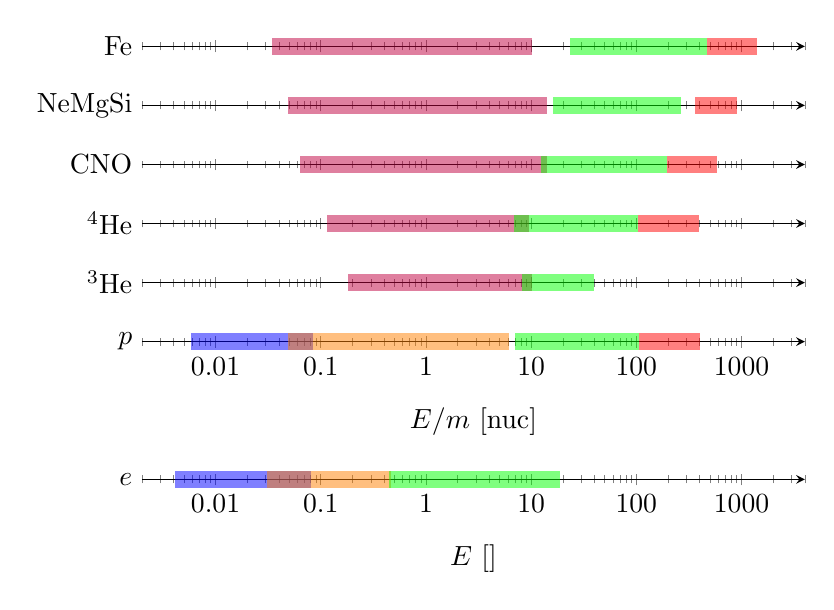
\begin{tikzpicture}
	\def\xmin{0.002}
	\def\xmax{4000}

	% EPT energy ranges, based on calibration as of 2020-10-01
	% ELECTRONS
	\begin{semilogxaxis}[xmin=\xmin, xmax=\xmax, axis x line=middle, hide y axis, ymin=-2,ymax=2,
					 height=2cm, width=10cm,
					 xlabel={$E$ [\si{\mega\electronvolt}]},
					 x label style={at={(axis description cs:0.5,-1.2)},anchor=north},clip=false,
					 log ticks with fixed point, x tick label style={/pgf/number format/1000 sep={}},yshift=0.25cm]
		\fill[blue, opacity=0.5] (axis cs:0.0041, -1) rectangle (axis cs:0.080, 1);
		\fill[orange, opacity=0.5] (axis cs:0.031, -1) rectangle (axis cs:0.47, 1);
		\fill[green, opacity=0.5] (axis cs:0.45, -1) rectangle (axis cs:18.8, 1);
		\node[left] at (axis cs:\xmin, 0) {$e$};
	\end{semilogxaxis}
	
	% PROTONS
	\begin{semilogxaxis}[xmin=\xmin, xmax=\xmax, axis x line=middle, hide y axis, ymin=-2,ymax=2,
	height=2cm, width=10cm, 
	xlabel={$E/m$ [\si{\mega\electronvolt\per nuc}]},
	x label style={at={(axis description cs:0.5,-1.2)},anchor=north},
	yshift=2cm, clip=false,
	log ticks with fixed point, x tick label style={/pgf/number format/1000 sep={}}]
		\fill[blue, opacity=0.5] (axis cs:0.0058, -1) rectangle (axis cs:0.085, 1);
		\fill[orange, opacity=0.5] (axis cs:0.049, -1) rectangle (axis cs:6.1, 1);
		\fill[green, opacity=0.5] (axis cs:7.0, -1) rectangle (axis cs:105, 1);
		\fill[red, opacity=0.5] (axis cs:105, -1) rectangle (axis cs:401.13, 1);
		%\fill[purple, opacity=0.5] (axis cs:0.24, 1) rectangle (axis cs:9.4, 3);
		\node[left] at (axis cs:\xmin, 0) {$p$};
	\end{semilogxaxis}
	
	% 3He
	\begin{semilogxaxis}[xmin=\xmin, xmax=\xmax, axis x line=middle, hide y axis, ymin=-2,ymax=2,
	height=2cm, width=10cm, xticklabels={,,},
	yshift=2.75cm, clip=false]
		\fill[purple, opacity=0.5] (axis cs:0.18, -1) rectangle (axis cs:10.2, 1);
		\fill[green, opacity=0.5] (axis cs:8.1, -1) rectangle (axis cs:39.7, 1);
		\node[left] at (axis cs:\xmin, 0) {$^3$He};
	\end{semilogxaxis}
	
	% 4He
	\begin{semilogxaxis}[xmin=\xmin, xmax=\xmax, axis x line=middle, hide y axis, ymin=-2,ymax=2,
	height=2cm, width=10cm, xticklabels={,,},
	yshift=3.5cm, clip=false]
		%\fill[orange, opacity=0.5] (axis cs:6.37, 1) rectangle (axis cs:24.51, 3);
		\fill[purple, opacity=0.5] (axis cs:0.115, -1) rectangle (axis cs:9.493, 1);
		\fill[green, opacity=0.5] (axis cs:6.877, -1) rectangle (axis cs:104, 1);
		\fill[red, opacity=0.5] (axis cs:104, -1) rectangle (axis cs:392.84, 1);
		\node[left] at (axis cs:\xmin, 0) {$^4$He};
	\end{semilogxaxis}
	
	% CNO
	\begin{semilogxaxis}[xmin=\xmin, xmax=\xmax, axis x line=middle, hide y axis, ymin=-2,ymax=2,
	height=2cm, width=10cm, xticklabels={,,},
	yshift=4.25cm, clip=false]
		\fill[purple, opacity=0.5] (axis cs:0.064, -1) rectangle (axis cs:14.13, 1);
		\fill[green, opacity=0.5] (axis cs:12.54, -1) rectangle (axis cs:197, 1);
		\fill[red, opacity=0.5] (axis cs:197, -1) rectangle (axis cs:578.37, 1);
		\node[left] at (axis cs:\xmin, 0) {CNO};
	\end{semilogxaxis}
	
	% NeMgSi
	\begin{semilogxaxis}[xmin=\xmin, xmax=\xmax, axis x line=middle, hide y axis, ymin=-2,ymax=2,
	height=2cm, width=10cm, xticklabels={,,},
	yshift=5cm, clip=false]
		\fill[purple, opacity=0.5] (axis cs:0.049, -1) rectangle (axis cs:14.13, 1);
		\fill[green, opacity=0.5] (axis cs:16.2, -1) rectangle (axis cs:268.42, 1);
		\fill[red, opacity=0.5] (axis cs:358, -1) rectangle (axis cs:915.03, 1);
		\node[left] at (axis cs:\xmin, 0) {NeMgSi};
	\end{semilogxaxis}
	
	% Fe
	\begin{semilogxaxis}[xmin=\xmin, xmax=\xmax, axis x line=middle, hide y axis, ymin=-2,ymax=2,
	height=2cm, width=10cm, xticklabels={,,},
	yshift=5.75cm, clip=false]
		\fill[purple, opacity=0.5] (axis cs:0.0346, -1) rectangle (axis cs:10.29, 1);
		\fill[green, opacity=0.5] (axis cs:23.66, -1) rectangle (axis cs:465.7, 1);
		\fill[red, opacity=0.5] (axis cs:465.8, -1) rectangle (axis cs:1388.40, 1);
		\node[left] at (axis cs:\xmin, 0) {Fe};
	\end{semilogxaxis}
\end{tikzpicture}
%\end{document}
% 	\caption[\acs{EPD} energy coverage]{Energy coverage of the different sensors in the \ac{SolO} \ac{EPD} suite for electrons and different ion species, based on the current science data products as of October 2020. This is an updated and enhanced version of Figure 3 from \citet{RodriguezPacheco-2019-EPD}. In the case of the CNO and NeMgSi groups, the responses for carbon and neon were taken as an example, the other species differ only slightly. For simplicity, \acs{SIS} protons, \acs{EPT} stopping helium as well as \acs{EPT} penetrating data products, which overlap with other measurements, are excluded from this plot. For the penetrating data products of \acs{HET}, the highest energy bin \citep[as given by][Appendix A]{Elftmann-2020-PhD} is not included, as its coverage extends to infinity.}
% 	\label{fig:epd_energy_ranges}
% \end{figure}
% The lowest energies of electrons and protons, from a few \si{\kilo\electronvolt} (slightly above the solar wind bulk) up to \SI{80}{\kilo\electronvolt}, are measured by the \ac{STEP} telescope, which is followed by the \ac{EPT} for medium energies up to $\sim\SI{6}{\mega\electronvolt}$ for protons and \SI{450}{\kilo\electronvolt} for electrons. Both \ac{EPT} and \ac{STEP} mainly measure electrons and protons, but cannot distinguish between protons and heavier ion species. Hence, they are supplemented with the \ac{SIS}, a time-of-flight based instrument that measures 12 ion species from H to Fe between \SI{14}{\kilo\electronvolt\per nuc} and \SI{20.5}{\mega\electronvolt\per nuc}. The highest energies of electrons and all ion species are covered by the \ac{HET}, whose measurements are, similarly to \ac{MSL}/\ac{RAD} (\autoref{sec:mslrad}), based on the $\dd E/\dd x$-$E$ method.

% The double-ended \ac{HET} sensor head is shown in Figure \ref{subfig:het-sensorhead-cad}. Two of these sensors are installed on the side decks of the \ac{SolO} spacecraft to provide four viewing directions: sunward, antisunward, north and south. The sunward and antisunward fields of view (\ac{HET} 1) are pointed \SI{35}{\degree} away from the radial direction within the ecliptic, which corresponds to the nominal Parker spiral direction, while the north and south fields of view (\ac{HET} 2) are pointed out of the ecliptic. The \ac{HET} telescopes each consist of four silicon solid-state detectors (A1, B1, B2, A2) and a bismuth germanium oxide (Bi$_4$Ge$_3$O$_{12}$, BGO) scintillator (C) in the center. This setup is similar to \ac{RAD}, though there is no second plastic scintillator for the detection of neutral particles.

% \begin{figure}
% 	\centering
% 	\subfloat[\acs{CAD} rendering of the \ac{HET} sensor head. Adapted from \citet{RodriguezPacheco-2019-EPD}, Fig. 31.]{
% 		\includegraphics[width=0.7\textwidth]{images/het_enhanced.png}
% 		\label{subfig:het-sensorhead-cad}
% 	}\\
% 	\subfloat[Schematic diagram of the \ac{HET} sensor head. Exemplary particle trajectories ending up in different data products are shown by the arrows: \textcolor{red}{stopping in B}, \textcolor{green}{stopping in C}, \textcolor{blue}{penetrating}, \textcolor{Aquamarine}{GCR channel}, \textcolor{orange}{C single counter}.]{
% 		%\documentclass{standalone}
%\usepackage[dvipsnames]{xcolor}
%\usepackage{tikz}
%\usepackage{amsmath}
%\usepackage{siunitx}

%\usetikzlibrary{calc}
%\usetikzlibrary{decorations.pathmorphing}

%\definecolor{light-gray}{gray}{0.9}

%\begin{document}
\begin{tikzpicture}[scale=0.4]
    \tikzset{%
        add/.style args={#1 and #2}{
            to path={%
                ($(\tikztostart)!-#1!(\tikztotarget)$)--($(\tikztotarget)!-#2!(\tikztostart)$)%
                \tikztonodes},add/.default={.2 and .2}}
    }   
    
    \def\Sithickness{0.05}
    
    % A1
    \draw[fill=light-gray] (-\Sithickness, -0.87) rectangle (\Sithickness, 0.87) node[above,yshift=2mm]{\small A1};
    \draw (-\Sithickness, -0.4) -- (\Sithickness, -0.4);
    \draw (-\Sithickness, 0.4) -- (\Sithickness, 0.4);
    
    % B1
    \draw[fill=light-gray] (4.4-\Sithickness, -1.82) rectangle (4.4+\Sithickness, 1.82) node[above]{\small B1};
    \draw (4.4-\Sithickness, -0.4) -- (4.4+\Sithickness, -0.4);
    \draw (4.4-\Sithickness, 0.4) -- (4.4+\Sithickness, 0.4);
    \draw (4.4-\Sithickness, -0.87) -- (4.4+\Sithickness, -0.87);
    \draw (4.4-\Sithickness, 0.87) -- (4.4+\Sithickness, 0.87);
    
    % C
    \draw[fill=light-gray] (4.635, -1.75) rectangle ++(2, 3.5);
    \node[above, yshift=0.5mm] at (5.635, 1.75) {\small C};
    
    % B2
    \draw[fill=light-gray] (6.9-\Sithickness, -1.82) rectangle (6.9+\Sithickness, 1.82) node[above]{\small B2};
    \draw (6.9-\Sithickness, -0.4) -- (6.9+\Sithickness, -0.4);
    \draw (6.9-\Sithickness, 0.4) -- (6.9+\Sithickness, 0.4);
    \draw (6.9-\Sithickness, -0.87) -- (6.9+\Sithickness, -0.87);
    \draw (6.9-\Sithickness, 0.87) -- (6.9+\Sithickness, 0.87);
    
    % A2
    \draw[fill=light-gray] (11.3-\Sithickness, -0.87) rectangle (11.3+\Sithickness, 0.87) node[above,yshift=2mm]{\small A2};
    \draw (11.3-\Sithickness, -0.4) -- (11.3+\Sithickness, -0.4);
    \draw (11.3-\Sithickness, 0.4) -- (11.3+\Sithickness, 0.4);
    
    % FOV
    \draw[add=0.1 and 0, dashed, opacity=0.5] (0, -0.87) to (6.9, 1.82);
    \draw[add=0.1 and 0, dashed, opacity=0.5] (0, 0.87) to (6.9, -1.82);
    \draw[add=0.1 and 0, dashed, opacity=0.5] (11.3, -0.87) to (4.4, 1.82);
    \draw[add=0.1 and 0, dashed, opacity=0.5] (11.3, 0.87) to (4.4, -1.82);
    
    \draw[|<->|] (0, 0.87) ++ (180-21.45:0.5) arc (180-21.45:180+21.45:2.4+0.48) node[midway, left] {\small\SI{42.9}{\degree}};
    

    \draw[thick, red, -latex] (-0.2, 0.2) -- (4.4, 0.5);
    \draw[thick, green, -latex] (-0.2, 0) -- (5.7, 0.1);
    \draw[thick, blue, -latex] (-0.2, -0.2) -- (11.5, -0.5);
    \uncover<2->{
        \draw[thick, Aquamarine, -latex] (2.5, 2) -- (8.4, -2);
        \draw[thick, orange, -latex] (5.635, -2.3) -- (5.635, -1);
    }
\end{tikzpicture}
%\end{document}
% 		\label{subfig:het-sensorhead-diagram}
% 	}
% 	\caption[\acs{HET} sensor head]{\acs{HET} sensor head}
% 	\label{fig:het-sensorhead}
% \end{figure}

% Charged particles that enter through one of the A detectors and then stop in B or C are measured in the \ac{HET} data products for stopping particles, which are defined using the ABnC and ABC coincidence conditions (as shown in red and green in \autoref{subfig:het-sensorhead-diagram}). These particles are fully analyzed using the $\dd E/\dd x$-$E$ method, i.e. their primary energy and charge can be directly determined.
% Ions with higher energies (e.g. $\gtrsim\SI{100}{\mega\electronvolt\per nuc}$ for protons and helium) penetrate the whole telescope (ABCBA coincidence, shown in blue in \autoref{subfig:het-sensorhead-diagram}). In this case, as with the penetrating particles in \ac{RAD}, the particles are not fully analyzed. Still, up to a few hundred \si{\mega\electronvolt\per nuc}, the particle direction and primary energy can be estimated based on the different \ac{LET} at each end of the telescope (e.g. in the A1 and A2 detectors).

% Similarly to \ac{RAD}, these energy-resolved stopping and penetrating particle data products are very useful for \ac{SEP} events as well as to calculate longterm \ac{GCR} spectra, but they do not have high enough count rates to study short-term variations of the \ac{GCR}. Alternatively, \ac{HET} also produces a data product using the BCB coincidence (irrespective of the A detectors, shown in turquoise in \autoref{subfig:het-sensorhead-diagram}), which significantly increases the opening angle at the cost of lower energy resolution and no separation of particle species. For this data product, only a 1D histogram of the energy deposit in C is stored. In addition, basic single detector count rates (level 1 trigger rates) without any coincidence conditions applied are available in \ac{HET}'s housekeeping data, which include particles entering \ac{HET} from any direction. In this case, the count rates for the C detector are best suited for measuring short-term variations due to the large volume of C. The response function of this single detector counter is derived in \autoref{chp:HETSimulation}.

% Further details about the design of the \ac{HET} instrument, the definition of its data products and their calibration can be found in \citet{Elftmann-2020-PhD}. 

% \section{Neutron monitor measurements}
% \label{sec:neutronmonitors}

% First developed in the 1950s \citep[see e.g.][]{Simpson-2000}, ground-based neutron monitors have historically been the most widely available instrument for the measurement of the cosmic ray flux at Earth. Neutron monitors measure secondary neutrons generated by the primary \ac{GCR} and \ac{SEP} particles in the Earth's atmosphere. They are typically large and heavy instruments, as one or more large tubes of lead are needed to achieve a sufficiently large detection efficiency for high-energy neutrons. Within a decade, such devices had been deployed at numerous locations around the globe, and many of them have been producing measurements almost continuously until the present day. Today, data from the global network of more than 50 neutron monitors \citep[e.g.][]{Moraal-2000} are archived at the \acl{NMDB}\acused{NMDB} \citep[\acs{NMDB},][]{Steigies-2009}\footnote{\url{https://www.nmdb.eu}}, and many of these stations are also providing realtime data through \ac{NMDB}.

% Similar to \ac{RAD} on Mars (\autoref{sec:mslrad}), neutron monitor measurements are influenced by the Earth's atmosphere, but also by the magnetic field, which is negligible at Mars. Thus, any cosmic ray particle needs a certain minimum energy, the so-called cutoff energy, to be able to pass through the magnetosphere and produce a secondary neutron in the atmosphere, which then reaches the ground and can be detected by a neutron monitor. The atmospheric effect is mainly dependent on the altitude as well as the atmospheric pressure, while the magnetospheric effect depends on the geographic location, particularly the latitude. At the poles, where the magnetic field lines are nearly vertical, the magnetic cutoff decreases to zero, and thus the atmospheric effect is dominant in this case.

% The cutoff energy is often also expressed in terms of a rigidity
% \begin{equation}
% 	R = \frac{pc}{q},
% \end{equation}
% a quantity which is given in units of volts (\si{V}). $p$ is the particle's momentum, $q$ its charge and $c$ the speed of light. The benefit of using rigidities instead of (kinetic) energies is that particles with the same rigidity also have the same gyroradius in the magnetic field independent of the particle species. Using relativistic relations, $R$ can be rewritten in terms of the particle's charge $q = Ze$, rest mass $m_0$ and kinetic energy $E_\text{kin}$ as:
% \begin{equation}
%     R = \frac{1}{Ze} \sqrt{E_\text{kin}(E_\text{kin} + 2 m_0 c^2)}
% \end{equation}
% \citep[see e.g.][for the detailed derivation]{Moraal-2013}, which approaches $R \approx E_\text{kin}/(Ze)$ for highly relativistic particles ($E_\text{kin}\gg m_0 c^2$). So, for example, a \SI{100}{\giga\electronvolt} proton ($Z=1$) has a rigidity of approximately \SI{100}{\giga\volt}.

% Magnetic cutoff rigidities and the resulting response functions for neutron monitors, which take both the magnetospheric and the atmospheric effect into account, have been calculated by e.g. \citet{Clem-Dorman-2000,Smart-Shea-2001,Smart-Shea-2008}. The South Pole Neutron Monitor, located at the geographic south pole (\SI{90}{\degree} S) and \SI{2820}{\meter} altitude --- next to the Amundsen-Scott research station --- is the most sensitive neutron monitor station, as its magnetic cutoff is negligible and the atmospheric cutoff is also lower than at sea level. This makes it especially well suited for the detection of \acp{FD}, as they typically have larger amplitudes at lower energies (see \autoref{sec:forbush}). The South Pole Neutron Monitor will be used multiple times in this thesis to provide \ac{FD} observations at Earth that can be compared to the Mars or \ac{SolO} data.

% In addition to using single neutron monitors, an inversion method has also been developed to reconstruct the variation of the \ac{GCR} flux at a certain rigidity above the atmosphere and magnetosphere from the global network of neutron monitors. This so-called \ac{GSM} produces results that are independent of the characteristics of a single neutron monitor station. It is described in detail by \citet{Belov2018}, and is used e.g. as a basis for the extensive catalog of Forbush decreases at Earth compiled by the Russian Space Weather Prediction Center (IZMIRAN)\footnote{\url{http://spaceweather.izmiran.ru/eng/dbs.html}}, which is also employed in this thesis for statistical studies in the publication by \citet{Forstner-2020}.

% \section{The STEREO Heliospheric Imagers}
% \label{sec:stereohi}

% Launched in 2006, the \acl{STEREO}\acused{STEREO} \citep[\acs{STEREO},][]{Russell-2008-STEREO} is a NASA mission that enabled a stereoscopic view of the Sun for the first time. It consists of two largely identical spacecraft that were placed in an orbit around the Sun at distances close to \SI{1}{\AU}, carrying both in situ and remote sensing instruments. The \ac{STEREO}-A (Ahead) spacecraft is placed a bit closer to the Sun than Earth, while \ac{STEREO}-B (Behind) is a bit farther away. This caused the two spacecraft to slowly drift away from Earth, as A orbits the Sun slightly faster than Earth, and B slightly slower. 5 years later, the spacecraft were separated by \SI{180}{\degree} in longitude, and this made it possible to observe all sides of the Sun (except the poles) simultaneously for the first time. In 2015, the two spacecraft reached a solar conjunction, passing behind the Sun as seen from Earth, and are coming closer to Earth again ever since. Their next close approach to Earth is expected in 2023, 17 years after launch.

% With a planned mission duration of only 2 years, the \ac{STEREO} spacecraft were never designed to survive a solar conjunction, during which communication with Earth is not possible for several months, so significant configuration changes were necessary in the flight software. Unfortunately, while testing the new configuration designed for the solar conjunction phase, communications with the \ac{STEREO}-B spacecraft were lost on October 1, 2014, so since this date, science data are only available from \ac{STEREO}-A. It is believed that this was due to a temporary failure of the star tracker coinciding with incorrect data transmitted from one of the gyroscopes, causing the spacecraft to start spinning while it fired its thrusters in an attempt to compensate for the perceived rotation \citep{Cox-2018}. In this state, the spacecraft battery drained quickly as the solar panels were pointed toward the Sun only for a fraction of the time. The communications link to the spacecraft was restored for a few weeks in 2016, but the following attempt to re-stabilize the spacecraft was unsuccessful and connection was lost again. Recovery will be re-attempted when \ac{STEREO}-B comes closer to Earth in the next few years.

% Apart from three in situ experiments investigating the local solar wind plasma, energetic particles, magnetic fields and radio waves, the scientific payload onboard the \ac{STEREO} spacecraft also includes the \acl{SECCHI}\acused{SECCHI} \citep[\acs{SECCHI},][]{Howard-2008-SECCHI}, a suite of remote sensing instruments consisting of five telescopes (\autoref{tab:secchi_telescopes}) with different fields of view (from the solar disk to almost \SI{90}{\degree}) and wavelengths (\ac{EUV} and visible light, ``white light''). The \ac{EUV} imager (EUVI) observes the solar disk directly in four different wavelength bands, while the white-light coronagraphs COR1 and COR2 use an occulting disk in their center to cover the solar disk and observe the surrounding corona. Similar types of instruments have already been available from the Earth point of view, e.g. on the \ac{SOHO} spacecraft launched in the 1990s and its predecessors.
% On the other hand, the \aclp{HI}\acused{HI} \citep[\acs{HI},][]{Eyles2009-STEREOHI} are a relatively new type of instrument that had first been demonstrated in 2003 with the Solar Mass Ejection Imager \citep[SMEI,][]{Eyles-2003-SMEI} onboard the \textit{Coriolis} spacecraft. These white-light telescopes provide a very wide field of view between \SI{4}{\degree} and \SI{88.7}{\degree} from the Sun in the ecliptic plane and up to $\pm\SI{35}{\degree}$ in the perpendicular direction. With these data, \acp{CME} can be directly tracked from near the Sun out into interplanetary space. In contrast to the other telescopes, the \acp{HI} have rectangular fields of view directed away from the Sun towards one side --- therefore, the \ac{STEREO} spacecraft are always rotated so that the \acp{HI} can best observe the Sun-Earth line.

% \begin{table}
%     \begin{tabular}{llll}
%         \toprule
%     	Telescope & Description                & Wavelength                                                                         & Field of view                   \\
%         \midrule
%     	EUVI      & \ac{EUV} imager & \SI{171}{\angstrom}, \SI{195}{\angstrom}, \SI{284}{\angstrom}, \SI{304}{\angstrom} & \SIrange{0}{1.7}{\solarradius}  \\
%     	COR1      & inner coronagraph          & white light                                                                        & \SIrange{1.4}{4}{\solarradius}  \\
%     	COR2      & outer coronagraph          & white light                                                                        & \SIrange{2.5}{15}{\solarradius} \\
%     	HI1       & heliospheric imager 1  & white light                                                                        & \SIrange{4}{24}{\degree}        \\
%     	HI2       & heliospheric imager 2  & white light                                                                        & \SIrange{18.7}{88.7}{\degree}       \\
%         \bottomrule
%     \end{tabular}
%     \caption[Properties of the \acs{STEREO} \acs{SECCHI} telescopes]{Properties of the \acs{STEREO} \acs{SECCHI} telescopes.}
%     \label{tab:secchi_telescopes}
% \end{table}

% \autoref{fig:secchifov} demonstrates the different fields of view of the \ac{SECCHI} instruments. This composite image, which was constructed using the SunPy software toolkit \citep{sunpy_community2020}, shows the April 15, 2020 \ac{CME} \citep[see also \autoref{chp:solo} /][]{Forstner-2021-SolO}, which has just entered the HI1 field of view at this time. In addition, signatures of four solar system planets (Venus, Earth, Jupiter and Saturn) can be seen in the \acp{HI} telescopes, as well as the diagonal band of the Milky Way in HI2. The near-vertical trails in the \ac{HI} images are an instrumental artifact caused by the high relative brightness of the planets and some stars in combination with the column-wise sensor readout and the lack of a mechanical shutter.

% \begin{figure}
%     \centering
%     %% Creator: Matplotlib, PGF backend
%%
%% To include the figure in your LaTeX document, write
%%   \input{<filename>.pgf}
%%
%% Make sure the required packages are loaded in your preamble
%%   \usepackage{pgf}
%%
%% and, on pdftex
%%   \usepackage[utf8]{inputenc}\DeclareUnicodeCharacter{2212}{-}
%%
%% or, on luatex and xetex
%%   \usepackage{unicode-math}
%%
%% Figures using additional raster images can only be included by \input if
%% they are in the same directory as the main LaTeX file. For loading figures
%% from other directories you can use the `import` package
%%   \usepackage{import}
%%
%% and then include the figures with
%%   \import{<path to file>}{<filename>.pgf}
%%
%% Matplotlib used the following preamble
%%   \usepackage{fontspec}
%%
\begingroup%
\makeatletter%
\begin{pgfpicture}%
\pgfpathrectangle{\pgfpointorigin}{\pgfqpoint{5.200000in}{3.500000in}}%
\pgfusepath{use as bounding box, clip}%
\begin{pgfscope}%
\pgfsetbuttcap%
\pgfsetmiterjoin%
\definecolor{currentfill}{rgb}{1.000000,1.000000,1.000000}%
\pgfsetfillcolor{currentfill}%
\pgfsetlinewidth{0.000000pt}%
\definecolor{currentstroke}{rgb}{1.000000,1.000000,1.000000}%
\pgfsetstrokecolor{currentstroke}%
\pgfsetdash{}{0pt}%
\pgfpathmoveto{\pgfqpoint{0.000000in}{0.000000in}}%
\pgfpathlineto{\pgfqpoint{5.200000in}{0.000000in}}%
\pgfpathlineto{\pgfqpoint{5.200000in}{3.500000in}}%
\pgfpathlineto{\pgfqpoint{0.000000in}{3.500000in}}%
\pgfpathclose%
\pgfusepath{fill}%
\end{pgfscope}%
\begin{pgfscope}%
\pgfsetbuttcap%
\pgfsetmiterjoin%
\definecolor{currentfill}{rgb}{1.000000,1.000000,1.000000}%
\pgfsetfillcolor{currentfill}%
\pgfsetlinewidth{0.000000pt}%
\definecolor{currentstroke}{rgb}{0.000000,0.000000,0.000000}%
\pgfsetstrokecolor{currentstroke}%
\pgfsetstrokeopacity{0.000000}%
\pgfsetdash{}{0pt}%
\pgfpathmoveto{\pgfqpoint{0.582966in}{0.478438in}}%
\pgfpathlineto{\pgfqpoint{5.065000in}{0.478438in}}%
\pgfpathlineto{\pgfqpoint{5.065000in}{3.355531in}}%
\pgfpathlineto{\pgfqpoint{0.582966in}{3.355531in}}%
\pgfpathclose%
\pgfusepath{fill}%
\end{pgfscope}%
\begin{pgfscope}%
\pgfpathrectangle{\pgfqpoint{0.582966in}{0.478438in}}{\pgfqpoint{4.482034in}{2.877093in}}%
\pgfusepath{clip}%
\pgfsys@transformshift{1.710883in}{0.478438in}%
\pgftext[left,bottom]{\includegraphics[interpolate=true,width=3.356667in,height=2.880000in]{plots/secchi_fov-img0.png}}%
\end{pgfscope}%
\begin{pgfscope}%
\pgfpathrectangle{\pgfqpoint{0.582966in}{0.478438in}}{\pgfqpoint{4.482034in}{2.877093in}}%
\pgfusepath{clip}%
\pgfsetbuttcap%
\pgfsetmiterjoin%
\pgfsetlinewidth{1.003750pt}%
\definecolor{currentstroke}{rgb}{0.000000,0.000000,0.000000}%
\pgfsetstrokecolor{currentstroke}%
\pgfsetdash{}{0pt}%
\pgfpathmoveto{\pgfqpoint{1.710883in}{0.478438in}}%
\pgfpathlineto{\pgfqpoint{5.065000in}{0.478438in}}%
\pgfpathlineto{\pgfqpoint{5.065000in}{3.355531in}}%
\pgfpathlineto{\pgfqpoint{1.710883in}{3.355531in}}%
\pgfpathclose%
\pgfusepath{stroke}%
\end{pgfscope}%
\begin{pgfscope}%
\definecolor{textcolor}{rgb}{0.000000,0.000000,0.000000}%
\pgfsetstrokecolor{textcolor}%
\pgfsetfillcolor{textcolor}%
\pgftext[x=1.809694in,y=0.577249in,left,base]{\color{textcolor}\rmfamily\fontsize{12.000000}{14.400000}\bfseries\selectfont HI2}%
\end{pgfscope}%
\begin{pgfscope}%
\pgfsetbuttcap%
\pgfsetroundjoin%
\definecolor{currentfill}{rgb}{0.000000,0.000000,0.000000}%
\pgfsetfillcolor{currentfill}%
\pgfsetlinewidth{0.803000pt}%
\definecolor{currentstroke}{rgb}{0.000000,0.000000,0.000000}%
\pgfsetstrokecolor{currentstroke}%
\pgfsetdash{}{0pt}%
\pgfsys@defobject{currentmarker}{\pgfqpoint{0.000000in}{-0.048611in}}{\pgfqpoint{0.000000in}{0.000000in}}{%
\pgfpathmoveto{\pgfqpoint{0.000000in}{0.000000in}}%
\pgfpathlineto{\pgfqpoint{0.000000in}{-0.048611in}}%
\pgfusepath{stroke,fill}%
}%
\begin{pgfscope}%
\pgfsys@transformshift{0.790447in}{0.478438in}%
\pgfsys@useobject{currentmarker}{}%
\end{pgfscope}%
\end{pgfscope}%
\begin{pgfscope}%
\definecolor{textcolor}{rgb}{0.000000,0.000000,0.000000}%
\pgfsetstrokecolor{textcolor}%
\pgfsetfillcolor{textcolor}%
\pgftext[x=0.790447in,y=0.381216in,,top]{\color{textcolor}\rmfamily\fontsize{9.000000}{10.800000}\selectfont 0}%
\end{pgfscope}%
\begin{pgfscope}%
\pgfsetbuttcap%
\pgfsetroundjoin%
\definecolor{currentfill}{rgb}{0.000000,0.000000,0.000000}%
\pgfsetfillcolor{currentfill}%
\pgfsetlinewidth{0.803000pt}%
\definecolor{currentstroke}{rgb}{0.000000,0.000000,0.000000}%
\pgfsetstrokecolor{currentstroke}%
\pgfsetdash{}{0pt}%
\pgfsys@defobject{currentmarker}{\pgfqpoint{0.000000in}{-0.048611in}}{\pgfqpoint{0.000000in}{0.000000in}}{%
\pgfpathmoveto{\pgfqpoint{0.000000in}{0.000000in}}%
\pgfpathlineto{\pgfqpoint{0.000000in}{-0.048611in}}%
\pgfusepath{stroke,fill}%
}%
\begin{pgfscope}%
\pgfsys@transformshift{1.284501in}{0.478438in}%
\pgfsys@useobject{currentmarker}{}%
\end{pgfscope}%
\end{pgfscope}%
\begin{pgfscope}%
\definecolor{textcolor}{rgb}{0.000000,0.000000,0.000000}%
\pgfsetstrokecolor{textcolor}%
\pgfsetfillcolor{textcolor}%
\pgftext[x=1.284501in,y=0.381216in,,top]{\color{textcolor}\rmfamily\fontsize{9.000000}{10.800000}\selectfont 10}%
\end{pgfscope}%
\begin{pgfscope}%
\pgfsetbuttcap%
\pgfsetroundjoin%
\definecolor{currentfill}{rgb}{0.000000,0.000000,0.000000}%
\pgfsetfillcolor{currentfill}%
\pgfsetlinewidth{0.803000pt}%
\definecolor{currentstroke}{rgb}{0.000000,0.000000,0.000000}%
\pgfsetstrokecolor{currentstroke}%
\pgfsetdash{}{0pt}%
\pgfsys@defobject{currentmarker}{\pgfqpoint{0.000000in}{-0.048611in}}{\pgfqpoint{0.000000in}{0.000000in}}{%
\pgfpathmoveto{\pgfqpoint{0.000000in}{0.000000in}}%
\pgfpathlineto{\pgfqpoint{0.000000in}{-0.048611in}}%
\pgfusepath{stroke,fill}%
}%
\begin{pgfscope}%
\pgfsys@transformshift{1.778554in}{0.478438in}%
\pgfsys@useobject{currentmarker}{}%
\end{pgfscope}%
\end{pgfscope}%
\begin{pgfscope}%
\definecolor{textcolor}{rgb}{0.000000,0.000000,0.000000}%
\pgfsetstrokecolor{textcolor}%
\pgfsetfillcolor{textcolor}%
\pgftext[x=1.778554in,y=0.381216in,,top]{\color{textcolor}\rmfamily\fontsize{9.000000}{10.800000}\selectfont 20}%
\end{pgfscope}%
\begin{pgfscope}%
\pgfsetbuttcap%
\pgfsetroundjoin%
\definecolor{currentfill}{rgb}{0.000000,0.000000,0.000000}%
\pgfsetfillcolor{currentfill}%
\pgfsetlinewidth{0.803000pt}%
\definecolor{currentstroke}{rgb}{0.000000,0.000000,0.000000}%
\pgfsetstrokecolor{currentstroke}%
\pgfsetdash{}{0pt}%
\pgfsys@defobject{currentmarker}{\pgfqpoint{0.000000in}{-0.048611in}}{\pgfqpoint{0.000000in}{0.000000in}}{%
\pgfpathmoveto{\pgfqpoint{0.000000in}{0.000000in}}%
\pgfpathlineto{\pgfqpoint{0.000000in}{-0.048611in}}%
\pgfusepath{stroke,fill}%
}%
\begin{pgfscope}%
\pgfsys@transformshift{2.272608in}{0.478438in}%
\pgfsys@useobject{currentmarker}{}%
\end{pgfscope}%
\end{pgfscope}%
\begin{pgfscope}%
\definecolor{textcolor}{rgb}{0.000000,0.000000,0.000000}%
\pgfsetstrokecolor{textcolor}%
\pgfsetfillcolor{textcolor}%
\pgftext[x=2.272608in,y=0.381216in,,top]{\color{textcolor}\rmfamily\fontsize{9.000000}{10.800000}\selectfont 30}%
\end{pgfscope}%
\begin{pgfscope}%
\pgfsetbuttcap%
\pgfsetroundjoin%
\definecolor{currentfill}{rgb}{0.000000,0.000000,0.000000}%
\pgfsetfillcolor{currentfill}%
\pgfsetlinewidth{0.803000pt}%
\definecolor{currentstroke}{rgb}{0.000000,0.000000,0.000000}%
\pgfsetstrokecolor{currentstroke}%
\pgfsetdash{}{0pt}%
\pgfsys@defobject{currentmarker}{\pgfqpoint{0.000000in}{-0.048611in}}{\pgfqpoint{0.000000in}{0.000000in}}{%
\pgfpathmoveto{\pgfqpoint{0.000000in}{0.000000in}}%
\pgfpathlineto{\pgfqpoint{0.000000in}{-0.048611in}}%
\pgfusepath{stroke,fill}%
}%
\begin{pgfscope}%
\pgfsys@transformshift{2.766662in}{0.478438in}%
\pgfsys@useobject{currentmarker}{}%
\end{pgfscope}%
\end{pgfscope}%
\begin{pgfscope}%
\definecolor{textcolor}{rgb}{0.000000,0.000000,0.000000}%
\pgfsetstrokecolor{textcolor}%
\pgfsetfillcolor{textcolor}%
\pgftext[x=2.766662in,y=0.381216in,,top]{\color{textcolor}\rmfamily\fontsize{9.000000}{10.800000}\selectfont 40}%
\end{pgfscope}%
\begin{pgfscope}%
\pgfsetbuttcap%
\pgfsetroundjoin%
\definecolor{currentfill}{rgb}{0.000000,0.000000,0.000000}%
\pgfsetfillcolor{currentfill}%
\pgfsetlinewidth{0.803000pt}%
\definecolor{currentstroke}{rgb}{0.000000,0.000000,0.000000}%
\pgfsetstrokecolor{currentstroke}%
\pgfsetdash{}{0pt}%
\pgfsys@defobject{currentmarker}{\pgfqpoint{0.000000in}{-0.048611in}}{\pgfqpoint{0.000000in}{0.000000in}}{%
\pgfpathmoveto{\pgfqpoint{0.000000in}{0.000000in}}%
\pgfpathlineto{\pgfqpoint{0.000000in}{-0.048611in}}%
\pgfusepath{stroke,fill}%
}%
\begin{pgfscope}%
\pgfsys@transformshift{3.260715in}{0.478438in}%
\pgfsys@useobject{currentmarker}{}%
\end{pgfscope}%
\end{pgfscope}%
\begin{pgfscope}%
\definecolor{textcolor}{rgb}{0.000000,0.000000,0.000000}%
\pgfsetstrokecolor{textcolor}%
\pgfsetfillcolor{textcolor}%
\pgftext[x=3.260715in,y=0.381216in,,top]{\color{textcolor}\rmfamily\fontsize{9.000000}{10.800000}\selectfont 50}%
\end{pgfscope}%
\begin{pgfscope}%
\pgfsetbuttcap%
\pgfsetroundjoin%
\definecolor{currentfill}{rgb}{0.000000,0.000000,0.000000}%
\pgfsetfillcolor{currentfill}%
\pgfsetlinewidth{0.803000pt}%
\definecolor{currentstroke}{rgb}{0.000000,0.000000,0.000000}%
\pgfsetstrokecolor{currentstroke}%
\pgfsetdash{}{0pt}%
\pgfsys@defobject{currentmarker}{\pgfqpoint{0.000000in}{-0.048611in}}{\pgfqpoint{0.000000in}{0.000000in}}{%
\pgfpathmoveto{\pgfqpoint{0.000000in}{0.000000in}}%
\pgfpathlineto{\pgfqpoint{0.000000in}{-0.048611in}}%
\pgfusepath{stroke,fill}%
}%
\begin{pgfscope}%
\pgfsys@transformshift{3.754769in}{0.478438in}%
\pgfsys@useobject{currentmarker}{}%
\end{pgfscope}%
\end{pgfscope}%
\begin{pgfscope}%
\definecolor{textcolor}{rgb}{0.000000,0.000000,0.000000}%
\pgfsetstrokecolor{textcolor}%
\pgfsetfillcolor{textcolor}%
\pgftext[x=3.754769in,y=0.381216in,,top]{\color{textcolor}\rmfamily\fontsize{9.000000}{10.800000}\selectfont 60}%
\end{pgfscope}%
\begin{pgfscope}%
\pgfsetbuttcap%
\pgfsetroundjoin%
\definecolor{currentfill}{rgb}{0.000000,0.000000,0.000000}%
\pgfsetfillcolor{currentfill}%
\pgfsetlinewidth{0.803000pt}%
\definecolor{currentstroke}{rgb}{0.000000,0.000000,0.000000}%
\pgfsetstrokecolor{currentstroke}%
\pgfsetdash{}{0pt}%
\pgfsys@defobject{currentmarker}{\pgfqpoint{0.000000in}{-0.048611in}}{\pgfqpoint{0.000000in}{0.000000in}}{%
\pgfpathmoveto{\pgfqpoint{0.000000in}{0.000000in}}%
\pgfpathlineto{\pgfqpoint{0.000000in}{-0.048611in}}%
\pgfusepath{stroke,fill}%
}%
\begin{pgfscope}%
\pgfsys@transformshift{4.248823in}{0.478438in}%
\pgfsys@useobject{currentmarker}{}%
\end{pgfscope}%
\end{pgfscope}%
\begin{pgfscope}%
\definecolor{textcolor}{rgb}{0.000000,0.000000,0.000000}%
\pgfsetstrokecolor{textcolor}%
\pgfsetfillcolor{textcolor}%
\pgftext[x=4.248823in,y=0.381216in,,top]{\color{textcolor}\rmfamily\fontsize{9.000000}{10.800000}\selectfont 70}%
\end{pgfscope}%
\begin{pgfscope}%
\pgfsetbuttcap%
\pgfsetroundjoin%
\definecolor{currentfill}{rgb}{0.000000,0.000000,0.000000}%
\pgfsetfillcolor{currentfill}%
\pgfsetlinewidth{0.803000pt}%
\definecolor{currentstroke}{rgb}{0.000000,0.000000,0.000000}%
\pgfsetstrokecolor{currentstroke}%
\pgfsetdash{}{0pt}%
\pgfsys@defobject{currentmarker}{\pgfqpoint{0.000000in}{-0.048611in}}{\pgfqpoint{0.000000in}{0.000000in}}{%
\pgfpathmoveto{\pgfqpoint{0.000000in}{0.000000in}}%
\pgfpathlineto{\pgfqpoint{0.000000in}{-0.048611in}}%
\pgfusepath{stroke,fill}%
}%
\begin{pgfscope}%
\pgfsys@transformshift{4.742876in}{0.478438in}%
\pgfsys@useobject{currentmarker}{}%
\end{pgfscope}%
\end{pgfscope}%
\begin{pgfscope}%
\definecolor{textcolor}{rgb}{0.000000,0.000000,0.000000}%
\pgfsetstrokecolor{textcolor}%
\pgfsetfillcolor{textcolor}%
\pgftext[x=4.742876in,y=0.381216in,,top]{\color{textcolor}\rmfamily\fontsize{9.000000}{10.800000}\selectfont 80}%
\end{pgfscope}%
\begin{pgfscope}%
\definecolor{textcolor}{rgb}{0.000000,0.000000,0.000000}%
\pgfsetstrokecolor{textcolor}%
\pgfsetfillcolor{textcolor}%
\pgftext[x=2.823983in,y=0.214660in,,top]{\color{textcolor}\rmfamily\fontsize{9.000000}{10.800000}\selectfont Helioprojective Longitude [°]}%
\end{pgfscope}%
\begin{pgfscope}%
\pgfsetbuttcap%
\pgfsetroundjoin%
\definecolor{currentfill}{rgb}{0.000000,0.000000,0.000000}%
\pgfsetfillcolor{currentfill}%
\pgfsetlinewidth{0.803000pt}%
\definecolor{currentstroke}{rgb}{0.000000,0.000000,0.000000}%
\pgfsetstrokecolor{currentstroke}%
\pgfsetdash{}{0pt}%
\pgfsys@defobject{currentmarker}{\pgfqpoint{-0.048611in}{0.000000in}}{\pgfqpoint{-0.000000in}{0.000000in}}{%
\pgfpathmoveto{\pgfqpoint{-0.000000in}{0.000000in}}%
\pgfpathlineto{\pgfqpoint{-0.048611in}{0.000000in}}%
\pgfusepath{stroke,fill}%
}%
\begin{pgfscope}%
\pgfsys@transformshift{0.582966in}{0.570008in}%
\pgfsys@useobject{currentmarker}{}%
\end{pgfscope}%
\end{pgfscope}%
\begin{pgfscope}%
\definecolor{textcolor}{rgb}{0.000000,0.000000,0.000000}%
\pgfsetstrokecolor{textcolor}%
\pgfsetfillcolor{textcolor}%
\pgftext[x=0.314369in, y=0.526633in, left, base]{\color{textcolor}\rmfamily\fontsize{9.000000}{10.800000}\selectfont -30}%
\end{pgfscope}%
\begin{pgfscope}%
\pgfsetbuttcap%
\pgfsetroundjoin%
\definecolor{currentfill}{rgb}{0.000000,0.000000,0.000000}%
\pgfsetfillcolor{currentfill}%
\pgfsetlinewidth{0.803000pt}%
\definecolor{currentstroke}{rgb}{0.000000,0.000000,0.000000}%
\pgfsetstrokecolor{currentstroke}%
\pgfsetdash{}{0pt}%
\pgfsys@defobject{currentmarker}{\pgfqpoint{-0.048611in}{0.000000in}}{\pgfqpoint{-0.000000in}{0.000000in}}{%
\pgfpathmoveto{\pgfqpoint{-0.000000in}{0.000000in}}%
\pgfpathlineto{\pgfqpoint{-0.048611in}{0.000000in}}%
\pgfusepath{stroke,fill}%
}%
\begin{pgfscope}%
\pgfsys@transformshift{0.582966in}{0.817035in}%
\pgfsys@useobject{currentmarker}{}%
\end{pgfscope}%
\end{pgfscope}%
\begin{pgfscope}%
\definecolor{textcolor}{rgb}{0.000000,0.000000,0.000000}%
\pgfsetstrokecolor{textcolor}%
\pgfsetfillcolor{textcolor}%
\pgftext[x=0.314369in, y=0.773660in, left, base]{\color{textcolor}\rmfamily\fontsize{9.000000}{10.800000}\selectfont -25}%
\end{pgfscope}%
\begin{pgfscope}%
\pgfsetbuttcap%
\pgfsetroundjoin%
\definecolor{currentfill}{rgb}{0.000000,0.000000,0.000000}%
\pgfsetfillcolor{currentfill}%
\pgfsetlinewidth{0.803000pt}%
\definecolor{currentstroke}{rgb}{0.000000,0.000000,0.000000}%
\pgfsetstrokecolor{currentstroke}%
\pgfsetdash{}{0pt}%
\pgfsys@defobject{currentmarker}{\pgfqpoint{-0.048611in}{0.000000in}}{\pgfqpoint{-0.000000in}{0.000000in}}{%
\pgfpathmoveto{\pgfqpoint{-0.000000in}{0.000000in}}%
\pgfpathlineto{\pgfqpoint{-0.048611in}{0.000000in}}%
\pgfusepath{stroke,fill}%
}%
\begin{pgfscope}%
\pgfsys@transformshift{0.582966in}{1.064061in}%
\pgfsys@useobject{currentmarker}{}%
\end{pgfscope}%
\end{pgfscope}%
\begin{pgfscope}%
\definecolor{textcolor}{rgb}{0.000000,0.000000,0.000000}%
\pgfsetstrokecolor{textcolor}%
\pgfsetfillcolor{textcolor}%
\pgftext[x=0.314369in, y=1.020686in, left, base]{\color{textcolor}\rmfamily\fontsize{9.000000}{10.800000}\selectfont -20}%
\end{pgfscope}%
\begin{pgfscope}%
\pgfsetbuttcap%
\pgfsetroundjoin%
\definecolor{currentfill}{rgb}{0.000000,0.000000,0.000000}%
\pgfsetfillcolor{currentfill}%
\pgfsetlinewidth{0.803000pt}%
\definecolor{currentstroke}{rgb}{0.000000,0.000000,0.000000}%
\pgfsetstrokecolor{currentstroke}%
\pgfsetdash{}{0pt}%
\pgfsys@defobject{currentmarker}{\pgfqpoint{-0.048611in}{0.000000in}}{\pgfqpoint{-0.000000in}{0.000000in}}{%
\pgfpathmoveto{\pgfqpoint{-0.000000in}{0.000000in}}%
\pgfpathlineto{\pgfqpoint{-0.048611in}{0.000000in}}%
\pgfusepath{stroke,fill}%
}%
\begin{pgfscope}%
\pgfsys@transformshift{0.582966in}{1.311088in}%
\pgfsys@useobject{currentmarker}{}%
\end{pgfscope}%
\end{pgfscope}%
\begin{pgfscope}%
\definecolor{textcolor}{rgb}{0.000000,0.000000,0.000000}%
\pgfsetstrokecolor{textcolor}%
\pgfsetfillcolor{textcolor}%
\pgftext[x=0.314369in, y=1.267713in, left, base]{\color{textcolor}\rmfamily\fontsize{9.000000}{10.800000}\selectfont -15}%
\end{pgfscope}%
\begin{pgfscope}%
\pgfsetbuttcap%
\pgfsetroundjoin%
\definecolor{currentfill}{rgb}{0.000000,0.000000,0.000000}%
\pgfsetfillcolor{currentfill}%
\pgfsetlinewidth{0.803000pt}%
\definecolor{currentstroke}{rgb}{0.000000,0.000000,0.000000}%
\pgfsetstrokecolor{currentstroke}%
\pgfsetdash{}{0pt}%
\pgfsys@defobject{currentmarker}{\pgfqpoint{-0.048611in}{0.000000in}}{\pgfqpoint{-0.000000in}{0.000000in}}{%
\pgfpathmoveto{\pgfqpoint{-0.000000in}{0.000000in}}%
\pgfpathlineto{\pgfqpoint{-0.048611in}{0.000000in}}%
\pgfusepath{stroke,fill}%
}%
\begin{pgfscope}%
\pgfsys@transformshift{0.582966in}{1.558115in}%
\pgfsys@useobject{currentmarker}{}%
\end{pgfscope}%
\end{pgfscope}%
\begin{pgfscope}%
\definecolor{textcolor}{rgb}{0.000000,0.000000,0.000000}%
\pgfsetstrokecolor{textcolor}%
\pgfsetfillcolor{textcolor}%
\pgftext[x=0.314369in, y=1.514740in, left, base]{\color{textcolor}\rmfamily\fontsize{9.000000}{10.800000}\selectfont -10}%
\end{pgfscope}%
\begin{pgfscope}%
\pgfsetbuttcap%
\pgfsetroundjoin%
\definecolor{currentfill}{rgb}{0.000000,0.000000,0.000000}%
\pgfsetfillcolor{currentfill}%
\pgfsetlinewidth{0.803000pt}%
\definecolor{currentstroke}{rgb}{0.000000,0.000000,0.000000}%
\pgfsetstrokecolor{currentstroke}%
\pgfsetdash{}{0pt}%
\pgfsys@defobject{currentmarker}{\pgfqpoint{-0.048611in}{0.000000in}}{\pgfqpoint{-0.000000in}{0.000000in}}{%
\pgfpathmoveto{\pgfqpoint{-0.000000in}{0.000000in}}%
\pgfpathlineto{\pgfqpoint{-0.048611in}{0.000000in}}%
\pgfusepath{stroke,fill}%
}%
\begin{pgfscope}%
\pgfsys@transformshift{0.582966in}{1.805142in}%
\pgfsys@useobject{currentmarker}{}%
\end{pgfscope}%
\end{pgfscope}%
\begin{pgfscope}%
\definecolor{textcolor}{rgb}{0.000000,0.000000,0.000000}%
\pgfsetstrokecolor{textcolor}%
\pgfsetfillcolor{textcolor}%
\pgftext[x=0.378619in, y=1.761767in, left, base]{\color{textcolor}\rmfamily\fontsize{9.000000}{10.800000}\selectfont -5}%
\end{pgfscope}%
\begin{pgfscope}%
\pgfsetbuttcap%
\pgfsetroundjoin%
\definecolor{currentfill}{rgb}{0.000000,0.000000,0.000000}%
\pgfsetfillcolor{currentfill}%
\pgfsetlinewidth{0.803000pt}%
\definecolor{currentstroke}{rgb}{0.000000,0.000000,0.000000}%
\pgfsetstrokecolor{currentstroke}%
\pgfsetdash{}{0pt}%
\pgfsys@defobject{currentmarker}{\pgfqpoint{-0.048611in}{0.000000in}}{\pgfqpoint{-0.000000in}{0.000000in}}{%
\pgfpathmoveto{\pgfqpoint{-0.000000in}{0.000000in}}%
\pgfpathlineto{\pgfqpoint{-0.048611in}{0.000000in}}%
\pgfusepath{stroke,fill}%
}%
\begin{pgfscope}%
\pgfsys@transformshift{0.582966in}{2.052169in}%
\pgfsys@useobject{currentmarker}{}%
\end{pgfscope}%
\end{pgfscope}%
\begin{pgfscope}%
\definecolor{textcolor}{rgb}{0.000000,0.000000,0.000000}%
\pgfsetstrokecolor{textcolor}%
\pgfsetfillcolor{textcolor}%
\pgftext[x=0.421494in, y=2.008794in, left, base]{\color{textcolor}\rmfamily\fontsize{9.000000}{10.800000}\selectfont 0}%
\end{pgfscope}%
\begin{pgfscope}%
\pgfsetbuttcap%
\pgfsetroundjoin%
\definecolor{currentfill}{rgb}{0.000000,0.000000,0.000000}%
\pgfsetfillcolor{currentfill}%
\pgfsetlinewidth{0.803000pt}%
\definecolor{currentstroke}{rgb}{0.000000,0.000000,0.000000}%
\pgfsetstrokecolor{currentstroke}%
\pgfsetdash{}{0pt}%
\pgfsys@defobject{currentmarker}{\pgfqpoint{-0.048611in}{0.000000in}}{\pgfqpoint{-0.000000in}{0.000000in}}{%
\pgfpathmoveto{\pgfqpoint{-0.000000in}{0.000000in}}%
\pgfpathlineto{\pgfqpoint{-0.048611in}{0.000000in}}%
\pgfusepath{stroke,fill}%
}%
\begin{pgfscope}%
\pgfsys@transformshift{0.582966in}{2.299196in}%
\pgfsys@useobject{currentmarker}{}%
\end{pgfscope}%
\end{pgfscope}%
\begin{pgfscope}%
\definecolor{textcolor}{rgb}{0.000000,0.000000,0.000000}%
\pgfsetstrokecolor{textcolor}%
\pgfsetfillcolor{textcolor}%
\pgftext[x=0.421494in, y=2.255821in, left, base]{\color{textcolor}\rmfamily\fontsize{9.000000}{10.800000}\selectfont 5}%
\end{pgfscope}%
\begin{pgfscope}%
\pgfsetbuttcap%
\pgfsetroundjoin%
\definecolor{currentfill}{rgb}{0.000000,0.000000,0.000000}%
\pgfsetfillcolor{currentfill}%
\pgfsetlinewidth{0.803000pt}%
\definecolor{currentstroke}{rgb}{0.000000,0.000000,0.000000}%
\pgfsetstrokecolor{currentstroke}%
\pgfsetdash{}{0pt}%
\pgfsys@defobject{currentmarker}{\pgfqpoint{-0.048611in}{0.000000in}}{\pgfqpoint{-0.000000in}{0.000000in}}{%
\pgfpathmoveto{\pgfqpoint{-0.000000in}{0.000000in}}%
\pgfpathlineto{\pgfqpoint{-0.048611in}{0.000000in}}%
\pgfusepath{stroke,fill}%
}%
\begin{pgfscope}%
\pgfsys@transformshift{0.582966in}{2.546222in}%
\pgfsys@useobject{currentmarker}{}%
\end{pgfscope}%
\end{pgfscope}%
\begin{pgfscope}%
\definecolor{textcolor}{rgb}{0.000000,0.000000,0.000000}%
\pgfsetstrokecolor{textcolor}%
\pgfsetfillcolor{textcolor}%
\pgftext[x=0.357244in, y=2.502847in, left, base]{\color{textcolor}\rmfamily\fontsize{9.000000}{10.800000}\selectfont 10}%
\end{pgfscope}%
\begin{pgfscope}%
\pgfsetbuttcap%
\pgfsetroundjoin%
\definecolor{currentfill}{rgb}{0.000000,0.000000,0.000000}%
\pgfsetfillcolor{currentfill}%
\pgfsetlinewidth{0.803000pt}%
\definecolor{currentstroke}{rgb}{0.000000,0.000000,0.000000}%
\pgfsetstrokecolor{currentstroke}%
\pgfsetdash{}{0pt}%
\pgfsys@defobject{currentmarker}{\pgfqpoint{-0.048611in}{0.000000in}}{\pgfqpoint{-0.000000in}{0.000000in}}{%
\pgfpathmoveto{\pgfqpoint{-0.000000in}{0.000000in}}%
\pgfpathlineto{\pgfqpoint{-0.048611in}{0.000000in}}%
\pgfusepath{stroke,fill}%
}%
\begin{pgfscope}%
\pgfsys@transformshift{0.582966in}{2.793249in}%
\pgfsys@useobject{currentmarker}{}%
\end{pgfscope}%
\end{pgfscope}%
\begin{pgfscope}%
\definecolor{textcolor}{rgb}{0.000000,0.000000,0.000000}%
\pgfsetstrokecolor{textcolor}%
\pgfsetfillcolor{textcolor}%
\pgftext[x=0.357244in, y=2.749874in, left, base]{\color{textcolor}\rmfamily\fontsize{9.000000}{10.800000}\selectfont 15}%
\end{pgfscope}%
\begin{pgfscope}%
\pgfsetbuttcap%
\pgfsetroundjoin%
\definecolor{currentfill}{rgb}{0.000000,0.000000,0.000000}%
\pgfsetfillcolor{currentfill}%
\pgfsetlinewidth{0.803000pt}%
\definecolor{currentstroke}{rgb}{0.000000,0.000000,0.000000}%
\pgfsetstrokecolor{currentstroke}%
\pgfsetdash{}{0pt}%
\pgfsys@defobject{currentmarker}{\pgfqpoint{-0.048611in}{0.000000in}}{\pgfqpoint{-0.000000in}{0.000000in}}{%
\pgfpathmoveto{\pgfqpoint{-0.000000in}{0.000000in}}%
\pgfpathlineto{\pgfqpoint{-0.048611in}{0.000000in}}%
\pgfusepath{stroke,fill}%
}%
\begin{pgfscope}%
\pgfsys@transformshift{0.582966in}{3.040276in}%
\pgfsys@useobject{currentmarker}{}%
\end{pgfscope}%
\end{pgfscope}%
\begin{pgfscope}%
\definecolor{textcolor}{rgb}{0.000000,0.000000,0.000000}%
\pgfsetstrokecolor{textcolor}%
\pgfsetfillcolor{textcolor}%
\pgftext[x=0.357244in, y=2.996901in, left, base]{\color{textcolor}\rmfamily\fontsize{9.000000}{10.800000}\selectfont 20}%
\end{pgfscope}%
\begin{pgfscope}%
\pgfsetbuttcap%
\pgfsetroundjoin%
\definecolor{currentfill}{rgb}{0.000000,0.000000,0.000000}%
\pgfsetfillcolor{currentfill}%
\pgfsetlinewidth{0.803000pt}%
\definecolor{currentstroke}{rgb}{0.000000,0.000000,0.000000}%
\pgfsetstrokecolor{currentstroke}%
\pgfsetdash{}{0pt}%
\pgfsys@defobject{currentmarker}{\pgfqpoint{-0.048611in}{0.000000in}}{\pgfqpoint{-0.000000in}{0.000000in}}{%
\pgfpathmoveto{\pgfqpoint{-0.000000in}{0.000000in}}%
\pgfpathlineto{\pgfqpoint{-0.048611in}{0.000000in}}%
\pgfusepath{stroke,fill}%
}%
\begin{pgfscope}%
\pgfsys@transformshift{0.582966in}{3.287303in}%
\pgfsys@useobject{currentmarker}{}%
\end{pgfscope}%
\end{pgfscope}%
\begin{pgfscope}%
\definecolor{textcolor}{rgb}{0.000000,0.000000,0.000000}%
\pgfsetstrokecolor{textcolor}%
\pgfsetfillcolor{textcolor}%
\pgftext[x=0.357244in, y=3.243928in, left, base]{\color{textcolor}\rmfamily\fontsize{9.000000}{10.800000}\selectfont 25}%
\end{pgfscope}%
\begin{pgfscope}%
\definecolor{textcolor}{rgb}{0.000000,0.000000,0.000000}%
\pgfsetstrokecolor{textcolor}%
\pgfsetfillcolor{textcolor}%
\pgftext[x=0.258813in,y=1.916985in,,bottom,rotate=90.000000]{\color{textcolor}\rmfamily\fontsize{9.000000}{10.800000}\selectfont Helioprojective Latitude [°]}%
\end{pgfscope}%
\begin{pgfscope}%
\pgfsetrectcap%
\pgfsetmiterjoin%
\pgfsetlinewidth{0.803000pt}%
\definecolor{currentstroke}{rgb}{0.000000,0.000000,0.000000}%
\pgfsetstrokecolor{currentstroke}%
\pgfsetdash{}{0pt}%
\pgfpathmoveto{\pgfqpoint{0.582966in}{0.478438in}}%
\pgfpathlineto{\pgfqpoint{0.582966in}{3.355531in}}%
\pgfusepath{stroke}%
\end{pgfscope}%
\begin{pgfscope}%
\pgfsetrectcap%
\pgfsetmiterjoin%
\pgfsetlinewidth{0.803000pt}%
\definecolor{currentstroke}{rgb}{0.000000,0.000000,0.000000}%
\pgfsetstrokecolor{currentstroke}%
\pgfsetdash{}{0pt}%
\pgfpathmoveto{\pgfqpoint{5.065000in}{0.478438in}}%
\pgfpathlineto{\pgfqpoint{5.065000in}{3.355531in}}%
\pgfusepath{stroke}%
\end{pgfscope}%
\begin{pgfscope}%
\pgfsetrectcap%
\pgfsetmiterjoin%
\pgfsetlinewidth{0.803000pt}%
\definecolor{currentstroke}{rgb}{0.000000,0.000000,0.000000}%
\pgfsetstrokecolor{currentstroke}%
\pgfsetdash{}{0pt}%
\pgfpathmoveto{\pgfqpoint{0.582966in}{0.478438in}}%
\pgfpathlineto{\pgfqpoint{5.065000in}{0.478438in}}%
\pgfusepath{stroke}%
\end{pgfscope}%
\begin{pgfscope}%
\pgfsetrectcap%
\pgfsetmiterjoin%
\pgfsetlinewidth{0.803000pt}%
\definecolor{currentstroke}{rgb}{0.000000,0.000000,0.000000}%
\pgfsetstrokecolor{currentstroke}%
\pgfsetdash{}{0pt}%
\pgfpathmoveto{\pgfqpoint{0.582966in}{3.355531in}}%
\pgfpathlineto{\pgfqpoint{5.065000in}{3.355531in}}%
\pgfusepath{stroke}%
\end{pgfscope}%
\begin{pgfscope}%
\pgfpathrectangle{\pgfqpoint{0.582966in}{0.478438in}}{\pgfqpoint{4.482034in}{2.877093in}}%
\pgfusepath{clip}%
\pgfsys@transformshift{0.944714in}{1.480627in}%
\pgftext[left,bottom]{\includegraphics[interpolate=true,width=1.066667in,height=1.046667in]{plots/secchi_fov-img1.png}}%
\end{pgfscope}%
\begin{pgfscope}%
\pgfpathrectangle{\pgfqpoint{0.582966in}{0.478438in}}{\pgfqpoint{4.482034in}{2.877093in}}%
\pgfusepath{clip}%
\pgfsetbuttcap%
\pgfsetmiterjoin%
\pgfsetlinewidth{1.003750pt}%
\definecolor{currentstroke}{rgb}{0.000000,0.000000,0.000000}%
\pgfsetstrokecolor{currentstroke}%
\pgfsetdash{}{0pt}%
\pgfpathmoveto{\pgfqpoint{0.944714in}{1.480627in}}%
\pgfpathlineto{\pgfqpoint{2.009720in}{1.480627in}}%
\pgfpathlineto{\pgfqpoint{2.009720in}{2.527109in}}%
\pgfpathlineto{\pgfqpoint{0.944714in}{2.527109in}}%
\pgfpathclose%
\pgfusepath{stroke}%
\end{pgfscope}%
\begin{pgfscope}%
\definecolor{textcolor}{rgb}{0.000000,0.000000,0.000000}%
\pgfsetstrokecolor{textcolor}%
\pgfsetfillcolor{textcolor}%
\pgftext[x=1.043525in,y=1.579438in,left,base]{\color{textcolor}\rmfamily\fontsize{12.000000}{14.400000}\bfseries\selectfont HI1}%
\end{pgfscope}%
\begin{pgfscope}%
\pgfpathrectangle{\pgfqpoint{0.582966in}{0.478438in}}{\pgfqpoint{4.482034in}{2.877093in}}%
\pgfusepath{clip}%
\pgfsetbuttcap%
\pgfsetmiterjoin%
\pgfsetlinewidth{1.003750pt}%
\definecolor{currentstroke}{rgb}{0.000000,0.000000,0.000000}%
\pgfsetstrokecolor{currentstroke}%
\pgfsetdash{}{0pt}%
\pgfpathmoveto{\pgfqpoint{1.901498in}{1.915773in}}%
\pgfpathcurveto{\pgfqpoint{1.914601in}{1.915773in}}{\pgfqpoint{1.927168in}{1.920979in}}{\pgfqpoint{1.936433in}{1.930244in}}%
\pgfpathcurveto{\pgfqpoint{1.945698in}{1.939509in}}{\pgfqpoint{1.950904in}{1.952076in}}{\pgfqpoint{1.950904in}{1.965179in}}%
\pgfpathcurveto{\pgfqpoint{1.950904in}{1.978281in}}{\pgfqpoint{1.945698in}{1.990849in}}{\pgfqpoint{1.936433in}{2.000114in}}%
\pgfpathcurveto{\pgfqpoint{1.927168in}{2.009378in}}{\pgfqpoint{1.914601in}{2.014584in}}{\pgfqpoint{1.901498in}{2.014584in}}%
\pgfpathcurveto{\pgfqpoint{1.888396in}{2.014584in}}{\pgfqpoint{1.875828in}{2.009378in}}{\pgfqpoint{1.866563in}{2.000114in}}%
\pgfpathcurveto{\pgfqpoint{1.857299in}{1.990849in}}{\pgfqpoint{1.852093in}{1.978281in}}{\pgfqpoint{1.852093in}{1.965179in}}%
\pgfpathcurveto{\pgfqpoint{1.852093in}{1.952076in}}{\pgfqpoint{1.857299in}{1.939509in}}{\pgfqpoint{1.866563in}{1.930244in}}%
\pgfpathcurveto{\pgfqpoint{1.875828in}{1.920979in}}{\pgfqpoint{1.888396in}{1.915773in}}{\pgfqpoint{1.901498in}{1.915773in}}%
\pgfpathclose%
\pgfusepath{stroke}%
\end{pgfscope}%
\begin{pgfscope}%
\pgfpathrectangle{\pgfqpoint{0.582966in}{0.478438in}}{\pgfqpoint{4.482034in}{2.877093in}}%
\pgfusepath{clip}%
\pgfsetbuttcap%
\pgfsetmiterjoin%
\pgfsetlinewidth{1.003750pt}%
\definecolor{currentstroke}{rgb}{0.000000,0.000000,0.000000}%
\pgfsetstrokecolor{currentstroke}%
\pgfsetdash{}{0pt}%
\pgfpathmoveto{\pgfqpoint{1.498857in}{1.942865in}}%
\pgfpathcurveto{\pgfqpoint{1.511960in}{1.942865in}}{\pgfqpoint{1.524527in}{1.948071in}}{\pgfqpoint{1.533792in}{1.957336in}}%
\pgfpathcurveto{\pgfqpoint{1.543057in}{1.966601in}}{\pgfqpoint{1.548263in}{1.979168in}}{\pgfqpoint{1.548263in}{1.992271in}}%
\pgfpathcurveto{\pgfqpoint{1.548263in}{2.005373in}}{\pgfqpoint{1.543057in}{2.017941in}}{\pgfqpoint{1.533792in}{2.027206in}}%
\pgfpathcurveto{\pgfqpoint{1.524527in}{2.036470in}}{\pgfqpoint{1.511960in}{2.041676in}}{\pgfqpoint{1.498857in}{2.041676in}}%
\pgfpathcurveto{\pgfqpoint{1.485755in}{2.041676in}}{\pgfqpoint{1.473187in}{2.036470in}}{\pgfqpoint{1.463922in}{2.027206in}}%
\pgfpathcurveto{\pgfqpoint{1.454658in}{2.017941in}}{\pgfqpoint{1.449452in}{2.005373in}}{\pgfqpoint{1.449452in}{1.992271in}}%
\pgfpathcurveto{\pgfqpoint{1.449452in}{1.979168in}}{\pgfqpoint{1.454658in}{1.966601in}}{\pgfqpoint{1.463922in}{1.957336in}}%
\pgfpathcurveto{\pgfqpoint{1.473187in}{1.948071in}}{\pgfqpoint{1.485755in}{1.942865in}}{\pgfqpoint{1.498857in}{1.942865in}}%
\pgfpathclose%
\pgfusepath{stroke}%
\end{pgfscope}%
\begin{pgfscope}%
\pgfpathrectangle{\pgfqpoint{0.582966in}{0.478438in}}{\pgfqpoint{4.482034in}{2.877093in}}%
\pgfusepath{clip}%
\pgfsetbuttcap%
\pgfsetmiterjoin%
\pgfsetlinewidth{1.003750pt}%
\definecolor{currentstroke}{rgb}{0.000000,0.000000,0.000000}%
\pgfsetstrokecolor{currentstroke}%
\pgfsetdash{}{0pt}%
\pgfpathmoveto{\pgfqpoint{3.163965in}{2.033916in}}%
\pgfpathcurveto{\pgfqpoint{3.177068in}{2.033916in}}{\pgfqpoint{3.189635in}{2.039122in}}{\pgfqpoint{3.198900in}{2.048386in}}%
\pgfpathcurveto{\pgfqpoint{3.208165in}{2.057651in}}{\pgfqpoint{3.213371in}{2.070219in}}{\pgfqpoint{3.213371in}{2.083321in}}%
\pgfpathcurveto{\pgfqpoint{3.213371in}{2.096424in}}{\pgfqpoint{3.208165in}{2.108991in}}{\pgfqpoint{3.198900in}{2.118256in}}%
\pgfpathcurveto{\pgfqpoint{3.189635in}{2.127521in}}{\pgfqpoint{3.177068in}{2.132727in}}{\pgfqpoint{3.163965in}{2.132727in}}%
\pgfpathcurveto{\pgfqpoint{3.150863in}{2.132727in}}{\pgfqpoint{3.138295in}{2.127521in}}{\pgfqpoint{3.129030in}{2.118256in}}%
\pgfpathcurveto{\pgfqpoint{3.119766in}{2.108991in}}{\pgfqpoint{3.114560in}{2.096424in}}{\pgfqpoint{3.114560in}{2.083321in}}%
\pgfpathcurveto{\pgfqpoint{3.114560in}{2.070219in}}{\pgfqpoint{3.119766in}{2.057651in}}{\pgfqpoint{3.129030in}{2.048386in}}%
\pgfpathcurveto{\pgfqpoint{3.138295in}{2.039122in}}{\pgfqpoint{3.150863in}{2.033916in}}{\pgfqpoint{3.163965in}{2.033916in}}%
\pgfpathclose%
\pgfusepath{stroke}%
\end{pgfscope}%
\begin{pgfscope}%
\pgfpathrectangle{\pgfqpoint{0.582966in}{0.478438in}}{\pgfqpoint{4.482034in}{2.877093in}}%
\pgfusepath{clip}%
\pgfsetbuttcap%
\pgfsetmiterjoin%
\pgfsetlinewidth{1.003750pt}%
\definecolor{currentstroke}{rgb}{0.000000,0.000000,0.000000}%
\pgfsetstrokecolor{currentstroke}%
\pgfsetdash{}{0pt}%
\pgfpathmoveto{\pgfqpoint{3.416141in}{1.913435in}}%
\pgfpathcurveto{\pgfqpoint{3.429243in}{1.913435in}}{\pgfqpoint{3.441811in}{1.918640in}}{\pgfqpoint{3.451075in}{1.927905in}}%
\pgfpathcurveto{\pgfqpoint{3.460340in}{1.937170in}}{\pgfqpoint{3.465546in}{1.949738in}}{\pgfqpoint{3.465546in}{1.962840in}}%
\pgfpathcurveto{\pgfqpoint{3.465546in}{1.975943in}}{\pgfqpoint{3.460340in}{1.988510in}}{\pgfqpoint{3.451075in}{1.997775in}}%
\pgfpathcurveto{\pgfqpoint{3.441811in}{2.007040in}}{\pgfqpoint{3.429243in}{2.012245in}}{\pgfqpoint{3.416141in}{2.012245in}}%
\pgfpathcurveto{\pgfqpoint{3.403038in}{2.012245in}}{\pgfqpoint{3.390470in}{2.007040in}}{\pgfqpoint{3.381206in}{1.997775in}}%
\pgfpathcurveto{\pgfqpoint{3.371941in}{1.988510in}}{\pgfqpoint{3.366735in}{1.975943in}}{\pgfqpoint{3.366735in}{1.962840in}}%
\pgfpathcurveto{\pgfqpoint{3.366735in}{1.949738in}}{\pgfqpoint{3.371941in}{1.937170in}}{\pgfqpoint{3.381206in}{1.927905in}}%
\pgfpathcurveto{\pgfqpoint{3.390470in}{1.918640in}}{\pgfqpoint{3.403038in}{1.913435in}}{\pgfqpoint{3.416141in}{1.913435in}}%
\pgfpathclose%
\pgfusepath{stroke}%
\end{pgfscope}%
\begin{pgfscope}%
\pgfsetbuttcap%
\pgfsetmiterjoin%
\definecolor{currentfill}{rgb}{1.000000,1.000000,1.000000}%
\pgfsetfillcolor{currentfill}%
\pgfsetlinewidth{1.003750pt}%
\definecolor{currentstroke}{rgb}{0.000000,0.000000,0.000000}%
\pgfsetstrokecolor{currentstroke}%
\pgfsetdash{}{0pt}%
\pgfpathmoveto{\pgfqpoint{1.689276in}{1.715221in}}%
\pgfpathlineto{\pgfqpoint{2.113721in}{1.715221in}}%
\pgfpathlineto{\pgfqpoint{2.113721in}{1.869443in}}%
\pgfpathlineto{\pgfqpoint{1.689276in}{1.869443in}}%
\pgfpathclose%
\pgfusepath{stroke,fill}%
\end{pgfscope}%
\begin{pgfscope}%
\definecolor{textcolor}{rgb}{0.000000,0.000000,0.000000}%
\pgfsetstrokecolor{textcolor}%
\pgfsetfillcolor{textcolor}%
\pgftext[x=1.901498in,y=1.841665in,,top]{\color{textcolor}\rmfamily\fontsize{8.000000}{9.600000}\selectfont Jupiter}%
\end{pgfscope}%
\begin{pgfscope}%
\pgfsetbuttcap%
\pgfsetmiterjoin%
\definecolor{currentfill}{rgb}{1.000000,1.000000,1.000000}%
\pgfsetfillcolor{currentfill}%
\pgfsetlinewidth{1.003750pt}%
\definecolor{currentstroke}{rgb}{0.000000,0.000000,0.000000}%
\pgfsetstrokecolor{currentstroke}%
\pgfsetdash{}{0pt}%
\pgfpathmoveto{\pgfqpoint{1.297302in}{2.088006in}}%
\pgfpathlineto{\pgfqpoint{1.700413in}{2.088006in}}%
\pgfpathlineto{\pgfqpoint{1.700413in}{2.242228in}}%
\pgfpathlineto{\pgfqpoint{1.297302in}{2.242228in}}%
\pgfpathclose%
\pgfusepath{stroke,fill}%
\end{pgfscope}%
\begin{pgfscope}%
\definecolor{textcolor}{rgb}{0.000000,0.000000,0.000000}%
\pgfsetstrokecolor{textcolor}%
\pgfsetfillcolor{textcolor}%
\pgftext[x=1.498857in,y=2.115784in,,bottom]{\color{textcolor}\rmfamily\fontsize{8.000000}{9.600000}\selectfont Saturn}%
\end{pgfscope}%
\begin{pgfscope}%
\pgfsetbuttcap%
\pgfsetmiterjoin%
\definecolor{currentfill}{rgb}{1.000000,1.000000,1.000000}%
\pgfsetfillcolor{currentfill}%
\pgfsetlinewidth{1.003750pt}%
\definecolor{currentstroke}{rgb}{0.000000,0.000000,0.000000}%
\pgfsetstrokecolor{currentstroke}%
\pgfsetdash{}{0pt}%
\pgfpathmoveto{\pgfqpoint{2.983521in}{2.179057in}}%
\pgfpathlineto{\pgfqpoint{3.344410in}{2.179057in}}%
\pgfpathlineto{\pgfqpoint{3.344410in}{2.333279in}}%
\pgfpathlineto{\pgfqpoint{2.983521in}{2.333279in}}%
\pgfpathclose%
\pgfusepath{stroke,fill}%
\end{pgfscope}%
\begin{pgfscope}%
\definecolor{textcolor}{rgb}{0.000000,0.000000,0.000000}%
\pgfsetstrokecolor{textcolor}%
\pgfsetfillcolor{textcolor}%
\pgftext[x=3.163965in,y=2.206835in,,bottom]{\color{textcolor}\rmfamily\fontsize{8.000000}{9.600000}\selectfont Venus}%
\end{pgfscope}%
\begin{pgfscope}%
\pgfsetbuttcap%
\pgfsetmiterjoin%
\definecolor{currentfill}{rgb}{1.000000,1.000000,1.000000}%
\pgfsetfillcolor{currentfill}%
\pgfsetlinewidth{1.003750pt}%
\definecolor{currentstroke}{rgb}{0.000000,0.000000,0.000000}%
\pgfsetstrokecolor{currentstroke}%
\pgfsetdash{}{0pt}%
\pgfpathmoveto{\pgfqpoint{3.239974in}{1.712882in}}%
\pgfpathlineto{\pgfqpoint{3.592307in}{1.712882in}}%
\pgfpathlineto{\pgfqpoint{3.592307in}{1.867104in}}%
\pgfpathlineto{\pgfqpoint{3.239974in}{1.867104in}}%
\pgfpathclose%
\pgfusepath{stroke,fill}%
\end{pgfscope}%
\begin{pgfscope}%
\definecolor{textcolor}{rgb}{0.000000,0.000000,0.000000}%
\pgfsetstrokecolor{textcolor}%
\pgfsetfillcolor{textcolor}%
\pgftext[x=3.416141in,y=1.839327in,,top]{\color{textcolor}\rmfamily\fontsize{8.000000}{9.600000}\selectfont Earth}%
\end{pgfscope}%
\begin{pgfscope}%
\pgfpathrectangle{\pgfqpoint{0.582966in}{0.478438in}}{\pgfqpoint{4.482034in}{2.877093in}}%
\pgfusepath{clip}%
\pgfsys@transformshift{0.583333in}{1.846667in}%
\pgftext[left,bottom]{\includegraphics[interpolate=true,width=0.413333in,height=0.413333in]{plots/secchi_fov-img2.png}}%
\end{pgfscope}%
\end{pgfpicture}%
\makeatother%
\endgroup%

%     \caption[Fields of view of the \acs{STEREO} \acs{SECCHI} telescopes]{Composite image demonstrating the fields of view of the \ac{STEREO} \ac{SECCHI} telescopes EUVI, COR1, COR2 (blue, green and red areas on the left side), and HI1 and HI2. \ac{HI} images are shown as running difference images, while COR and EUVI are direct images. This image features the April 15, 2020 \ac{CME}, some planets as well as the Milky Way (diagonal band across the HI2 image).}
%     \label{fig:secchifov}
% \end{figure}

% \acp{CME} appear in the \ac{HI} telescopes due to Thomson scattering: Sunlight is scattered by free electrons in the solar wind plasma, and regions of enhanced density, such as \acp{CME} and the shocks driven by them, appear as brighter structures in the images. To make these transients more clearly visible, long exposure times on the order of 20 minutes to 1 hour are needed, and difference images are often used to further highlight the moving structures. In theory, the \SI{88.7}{\degree} field of view would allow the \acp{HI} to track \acp{CME} all the way out to Earth under most conditions. However, in practice, the \ac{CME} structures become more faint during the propagation as their density and velocity decreases. Also, \acp{CME} not directed towards Earth are not always covered by \ac{HI}, as these may also occur on the opposite side of the Sun (e.g. the left side of \autoref{fig:secchifov}).

% To routinely reconstruct the trajectories of \acp{CME} in the \ac{HI} observations, the 2D images are typically transformed into so-called J-maps, a technique which was originally developed by \citet{Sheeley-1999-JMap} and first applied to \ac{STEREO}-\ac{HI} data by \citet{Rouillard-2008-JMap}
% and \citet{Davies-2009}: After subtraction of backgrounds and the calculation of running difference images, a 1D slice is extracted from each \ac{HI} image in the time period of interest, usually close to the ecliptic plane. For each consecutive point in time, these slices are then rotated by \SI{90}{\degree} and concatenated into a new 2D plot, where time is on the x axis and the heliographic longitude, which in this case is named the \textit{elongation angle} $\epsilon$, is on the y axis. Moving structures, such as \ac{CME} or shock fronts, then appear as bright streaks in the J-map, which extend from the bottom (low elongation) out to larger elongations (see \autoref{subfig:jmap} for an example). Depending on the \ac{CME} direction and the evolution of its velocity, these structures can often resemble a (rotated) letter J, hence the corresponding naming of this type of plot. This is not the case in the example in \autoref{subfig:jmap}, as this slow \ac{CME} propagates at a nearly constant speed and produces a more or less straight line in the J-map.
% By tracing the structures in the J-map images, the time-elongation profile $\epsilon(t)$ can then easily be reconstructed.

% The more challenging part is to use this measurement to calculate the actual CME trajectory, i.e. the time profile of the radial distance $r(t)$ from the Sun. To solve this problem unambiguously, some assumptions need to be made, as the Thomson-scattered \ac{HI} image accumulates the electron density along the line of sight, which contains points at different heliospheric longitudes and radial distances. This means that the geometric shape of the \ac{CME} needs to be known to derive the position of the apex from the images. Multiple techniques have been developed to address this issue in different ways, starting with single-spacecraft approaches that also need to make assumptions about the CME longitude \citep{Howard-2006-PointP,Kahler-2007-FixedPhi,Lugaz-2009-HarmonicMean,Davies-2012-SSE}, followed by approaches that take into account the measurements from both \ac{STEREO} spacecraft at the same time to triangulate the CME location \citep{Liu-2010a-triangulation,Liu-2010b-triangulation,Lugaz-2010-TAS,Davies-2013-SSSE}. Of course, the latter can only be used for events observed by both spacecraft simultaneously, before the loss of connection to \ac{STEREO}-B in 2014. A detailed overview of these reconstruction methods and the corresponding mathematical expressions was given in Section 3.3.2 of \citet{Forstner-2018-masterthesis}.
% The single-spacecraft reconstruction methods are also summarized in Section 2.3 and Figure 2 of \citet{Forstner-2019}, which is reprinted in \autoref{chp:arrival_times} of this thesis.

% The \ac{HELCATS}\footnote{\url{https://www.helcats-fp7.eu/}} has systematically cataloged and analyzed all CMEs detected by the \ac{STEREO}-\ac{HI} telescopes and provides these data on their website. This database will serve as the basis for most \ac{HI}-related studies in this thesis. As an example, the images and J-map provided by \ac{HELCATS} for the April 15, 2020 CME observed by \ac{STEREO}-A are shown in \autoref{fig:hi_example}. The corresponding data and reconstruction results can be found under the ID \texttt{HCME\_A\_\_20200415\_01} in the \ac{HELCATS} catalogs.

% \begin{figure}
% 	\centering
% 	\subfloat[Direct image]{
% 		\includegraphics[width=0.4\textwidth]{images/HCME_A__20200415_01.png}
% 	}
% 	\subfloat[Running difference image]{
% 		\includegraphics[width=0.4\textwidth]{images/HCME_A__20200415_01_diff.png}
% 	}\\
% 	\subfloat[J-map]{
% 		\includegraphics[width=0.8\textwidth]{images/HCME_A__20200415_01_jmap.png}
% 		\label{subfig:jmap}
% 	}
% 	\caption[\acs{STEREO}-A \acs{HI} images of the April 15, 2020 CME]{\ac{STEREO}-A \ac{HI} images of the April 15, 2020 \ac{CME} generated by the \ac{HELCATS} project. In the J-map, the \ac{CME} trajectory was marked with red dots.}
% 	\label{fig:hi_example}
%\end{figure}

